\section{Detector performance with jet substructure variables}

In this section, we use several jet substructure variables to study the performance of detector with various detector cell sizes and c.m. energies.
%%By definition of Mann Whitney U test, if U value is close to 0.5, it means two distributions have similar compositions, and we can not distinguish them very well. On the other hand, if U value of two distributions are close to 0, it means both compositions of both distribution are much different from each other.\\

\subsection{$N$-subjettiness \label{sec:nsub}}
The variable $N$-subjettiness~\cite{Thaler:2010tr}, denoted by $\tau_N$, is designed to 
``count'' the number of subjet(s) in a large radius jet so to separate 
signal jets from decays of heavy bosons and background jets from QCD processes. 
The $\tau_N$ is the $\pt$-weighted angular distance between each jet 
constituent and the closest subjet axis: 
\begin{equation}\label{eq:Nsub_1}
\tau_{N}=\frac{1}{d_{0}}\sum_{k}p_{T,k} \mathrm{min}\{\Delta R_{1,k},\Delta R_{2,k},.....\Delta R_{N,k}\},
\end{equation}
with a normalization factor $d_0$: \[d_{0}=\sum_{k}p_{T,k} R_{0}.\] 
The $k$ runs over all constituent particles in a given large radius jet, 
$p_{T,k}$ is the transverse momentum of each individual constituent particle, 
$\Delta R_{j,k}=\sqrt{(\Delta y)^{2}+(\Delta \phi)^{2}}$ is the distance 
between the constituent particle $k$ and the candidate subjet axis $j$ in the 
$y-\phi$ plane. The $R_{0}$ is the characteristic jet radius used in 
the anti-$k_t$ jet algorithm. 

In this analysis, the anti-$k_t$ algorithm with $R=0.4$ (AK4) is first 
employed to reconstruct jets. The subjet axes are obtained by running the 
exclusive $k_{t}$ algorithm~\cite{Catani:246812} and reversing the last N clustering steps. 
Namely, when $\tau_N$ is computed, the $k_{t}$ algorithm is forced to return 
exactly $N$ jets. If a large radius jet has $N$ subjet(s), its $\tau_{N}$ is 
smaller than $\tau_{N-1}$. Therefore, in our analysis, 
the ratio of the $\tau_{N}$ variables, 
$\tau_{21}$ ($\tau_{2}/\tau_{1}$) and $\tau_{32}$ ($\tau_{3}/\tau_{2}$),  
are used to distinguish the one-prong background jets and 
the two-prong jets from W or the three-prong jets from top. 

We use the ROC curves as described in Section~\ref{sec:massana} to 
analyze the detector performance and determine the cell size that gives the 
best separation power to distinguish signal from background. 
Following the suggestion by Ref.~\cite{Dreyer:2018tjj}, the requirement on the 
soft drop mass with $\beta=0$ is applied before the study of $N$-subjettiness. 
For each detector configuration and c.m. energy, the soft drop mass selection 
is determined as follows. First, we look for the median bin of the soft drop 
mass histogram from simulated signal events as described in 
Section~\ref{sec:massana}.  Then, we compare the numbers of events in the 
bins adjacent to the medium bin (bin $i_\mathrm{med}-1$ 
and bin $i_\mathrm{med}+1$). The bin with larger number of events is added, 
in addition to the medium bin, to extend the mass window. The procedure is 
repeated until the window contains at least 75\% of the total number of signal 
events. 

In order to obtain the signal and background efficiencies, 
various ranges of $\tau_{21}$ and $\tau_{32}$ are scanned. 
Since some of the background distributions have long tails and leak into the 
signal-dominated region, we use the following method as suggested by the 
Pearson Lemma Method to determine the ranges of $\tau$ variables. 
First, we take the ratio of the signal to background $\tau_{21}$ ($\tau_{32}$) 
histograms. The boundaries of the bin (seed bin) with maximum signal to 
background ratio (S/N) give us the first range of $\tau$ selection: 
$x_\mathrm{low}^\mathrm{seedbin} < \tau_{21} <  x_\mathrm{high}^\mathrm{seedbin}$. 
Then, we compare the S/N in the bins adjacent to the seed bin. The bin with 
larger S/N is added, in addition to the seed bin, to extend the $\tau_{21}$ 
selection window. 
Every window has its corresponding $\epsilon_\mathrm{sig}$ and 
1/$\epsilon_\mathrm{bkg}$ and an ROC curve is mapped out. 

In addition to the ROC curves, we use the so-called "Mann-Whitney" test to 
quantify the detector performance. 
The value of Mann-Whitney is related to the integrated area under the ROC 
curve: if the value is bigger, it indicates the signal and background
 distributions have similar shapes and can not be well separated from 
each other. Vice versa, if the value is smaller, we can achieve a better 
signal and background separation. 

%First, we select the events in mass window by using SD with $\beta=0$ and 75$\%$ signal efficiency. Then, we find the highest ratio bin to be our seed bin. Next, we compare the left and right of ratio bin, and add the higher bin to be our width. Finally,  We can use this width to draw the ROC curves.\\
Figures~\ref{fig:Rawhit_05GeV_tau21_Dis} and~\ref{fig:Rawhit_05GeV_tau32_Dis} 
show the distributions of $\tau_{21}$ and $\tau_{32}$ for $\sqrt{s}=20$~TeV 
after applying the requirement on the soft drop mass. The signals considered are 
$Z'\rightarrow WW$ ($\tau_{21}$) and 
$Z' \rightarrow t\bar{t}$ ($\tau_{32}$). 
Figures~\ref{fig:Rawhit_05GeV_tau21_ROC} and~\ref{fig:Rawhit_05GeV_tau32_ROC} 
present the ROC curves from different detector cell sizes and c.m. energies, 
respectively. The smallest detector cell size ($1\times1~\mathrm{cm}^2$) 
does not have the best separation power. In fact, in some cases, 
the best separation power comes from a detector with bigger cell sizes 
($5\times5~\mathrm{cm}^2$ and $20\times20~\mathrm{cm}^2$).

Figures~\ref{fig:Rawhit_05GeV_total_Mann} (a) and (b) present the summary plots of $\tau_{21}$ and $\tau_{32}$ with various detector cell sizes and c.m. energies using Mann Whitney U test. For $\tau_{21}$ at smaller c.m. energies, when 
the cell size is smaller, the detector performance improves. However, 
when c.m. energy increases, no improvement 
is observed using the smallest detector cell size ($1\times1~\mathrm{cm}^2$). 
For $\tau_{32}$, the case is similar to  $\tau_{21}$. It is interesting to note that at very large  
c.m. energies, the large detector cell sizes ($5\times5~\mathrm{cm}^2$ and $20\times20~\mathrm{cm}^2$) have a 
better separation power than the smallest 
cell  size considered in this analysis. 

\subsection{Energy correlation function \label{sec:ecf}}
The energy correlation function (ECF)~\cite{Larkoski:2013eya} is defined as follows: 
%\begin{equation} \label{eq:ECF_Original}
%ECF(N,\beta)=\sum_{i_{1}<i_{2}<....<i_{N}\in J} (\prod_{a=1}^{N}E_{ia})(\prod_{%b=1}^{N-1}\prod_{c=b+1}^{N} \theta_{i_{b}i_{c}})^{\beta}, 
%\end{equation}
\begin{equation} \label{eq:ECF_Modified}
ECF(N,\beta)=\sum_{i_{1}<i_{2}<....<i_{N}\in J} \left(\prod_{a=1}^{N}p_{\mathrm{T}ia}\right)\left(\prod_{b=1}^{N-1}\prod_{c=b+1}^{N} R_{i_{b}i_{c}}\right)^{\beta},
\end{equation}
where the sum is looped all particles in the jet $J$, $\pt$ is the transverse 
momentum of each individual particle, and $R$ is the distance between two 
particles in the $y$-$\phi$ plane.  
In order to use a dimensionless variable, a parameter $r_{N}$ is defined:
\begin{equation} \label{eq:ECF_ratio}
r_{N}^{(\beta)}\equiv\frac{ECF(N+1,\beta)}{ECF(N,\beta)}.
\end{equation}

The idea of $r_N$ comes from N-subjettiness $\tau_N$. Both $r_N$ and $\tau_N$ 
are linear in the energy of the soft radiation for a system of $N$ partons 
with soft radiation. In general, if the system has N subjets, $ECF(N+1,\beta)$ 
should be significantly smaller than $ECF(N,\beta)$. Therefore, we can use this
 feature to distinguish jets with different numbers  of subjets. 
As in Section~\ref{sec:nsub}, the ratio $r_N/r_{N-1}$, denoted by $C_N$, 
(double ratios of ECFs) is used to study the detector performance: 
\begin{equation}
C_{N}^{(\beta)}\equiv\frac{r_{N}^{(\beta)}}{r_{N-1}^{(\beta)}}=\frac{ECF(N-1,\beta)ECF(N+1,\beta)}{ECF(N,\beta)^2}.
\end{equation}
In our analysis, we set $N=2$ and $\beta=1$ ($C_2^1$).

Figure~\ref{fig:Rawhit_05GeV_c2b1_Dis} presents the histograms of $C_{2}^{1}$ 
with $\sqrt{s}=20$~TeV after making the requirement on the soft drop mass. 
The signal considered is Z'$\rightarrow$WW. 
Figure~\ref{fig:Rawhit_05GeV_c2b1_ROC} shows the ROC curves from different 
detector cell sizes for each c.m. energy, respectively. One can see that 
the smallest detector cell size ($1\times1~\mathrm{cm}^2$) does not have the 
best signal/background separation power. 
Figure \ref{fig:Rawhit_05GeV_total_Mann}(c) summarizes the result of 
the Mann Whitney U test for $C_{2}^{1}$. When c.m. energy increases, 
no improvement is observed from detector with the smallest cell size. 


%%%%%%%%%%%% tau21
%25bins
\begin{figure}
\begin{center}
   \subfigure[20$\times$20 (cm$^2$)] {
   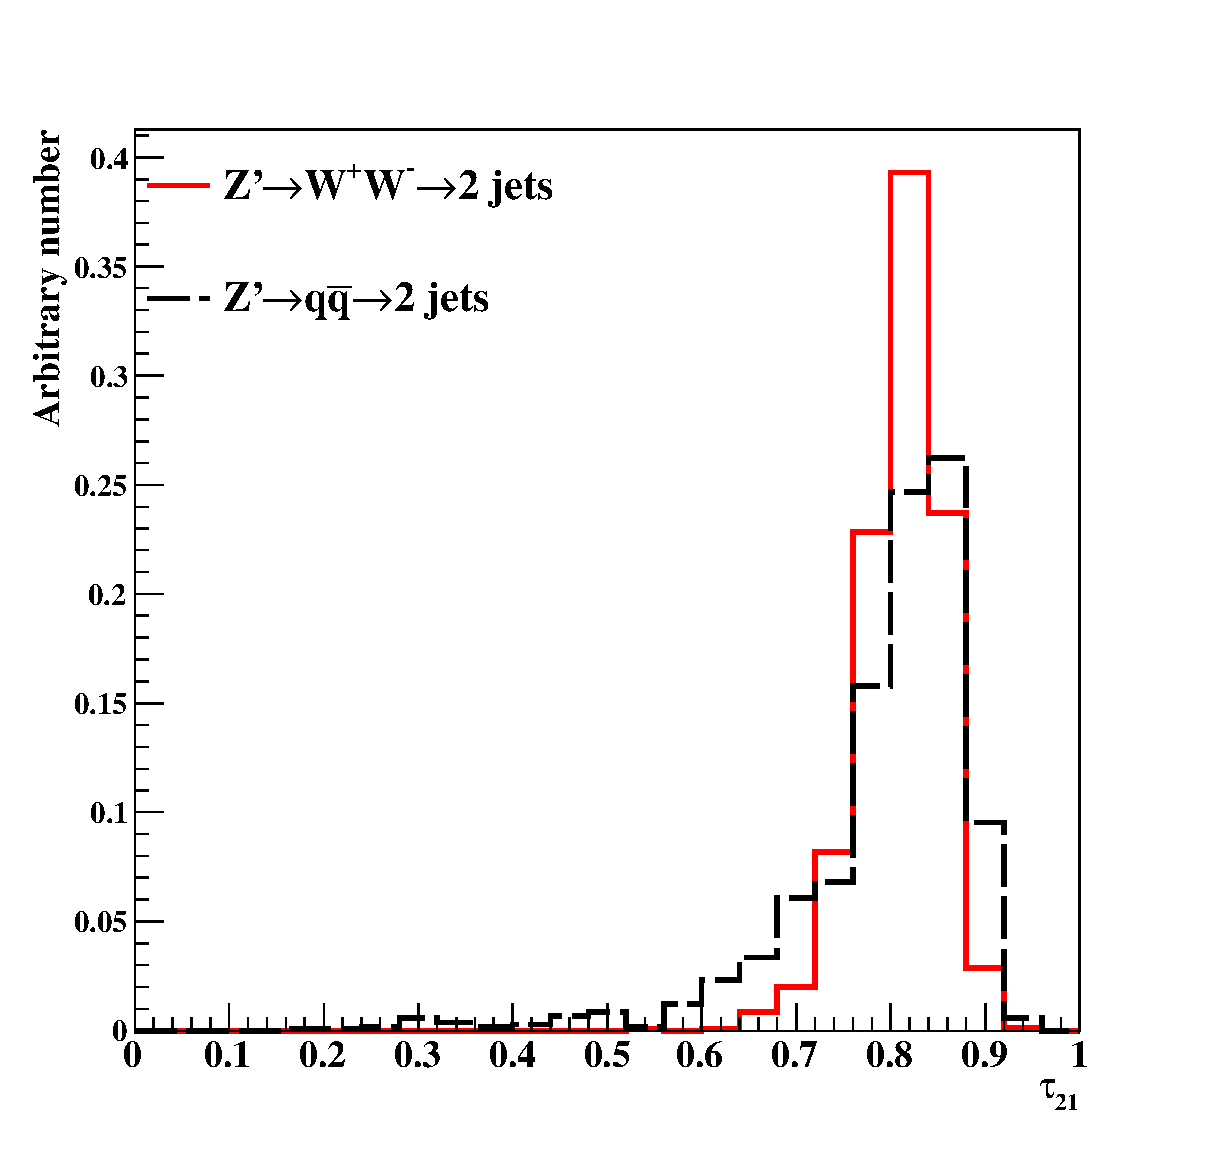
\includegraphics[width=0.3\textwidth]{h_Tau_C/Dis_Rawhit_05GeV_010_tau21_20tev_04_after_cut_Man_25_no_UOF_new_75pa_for_paper.eps}
   }
   \subfigure[5$\times$5 (cm$^2$)] {
   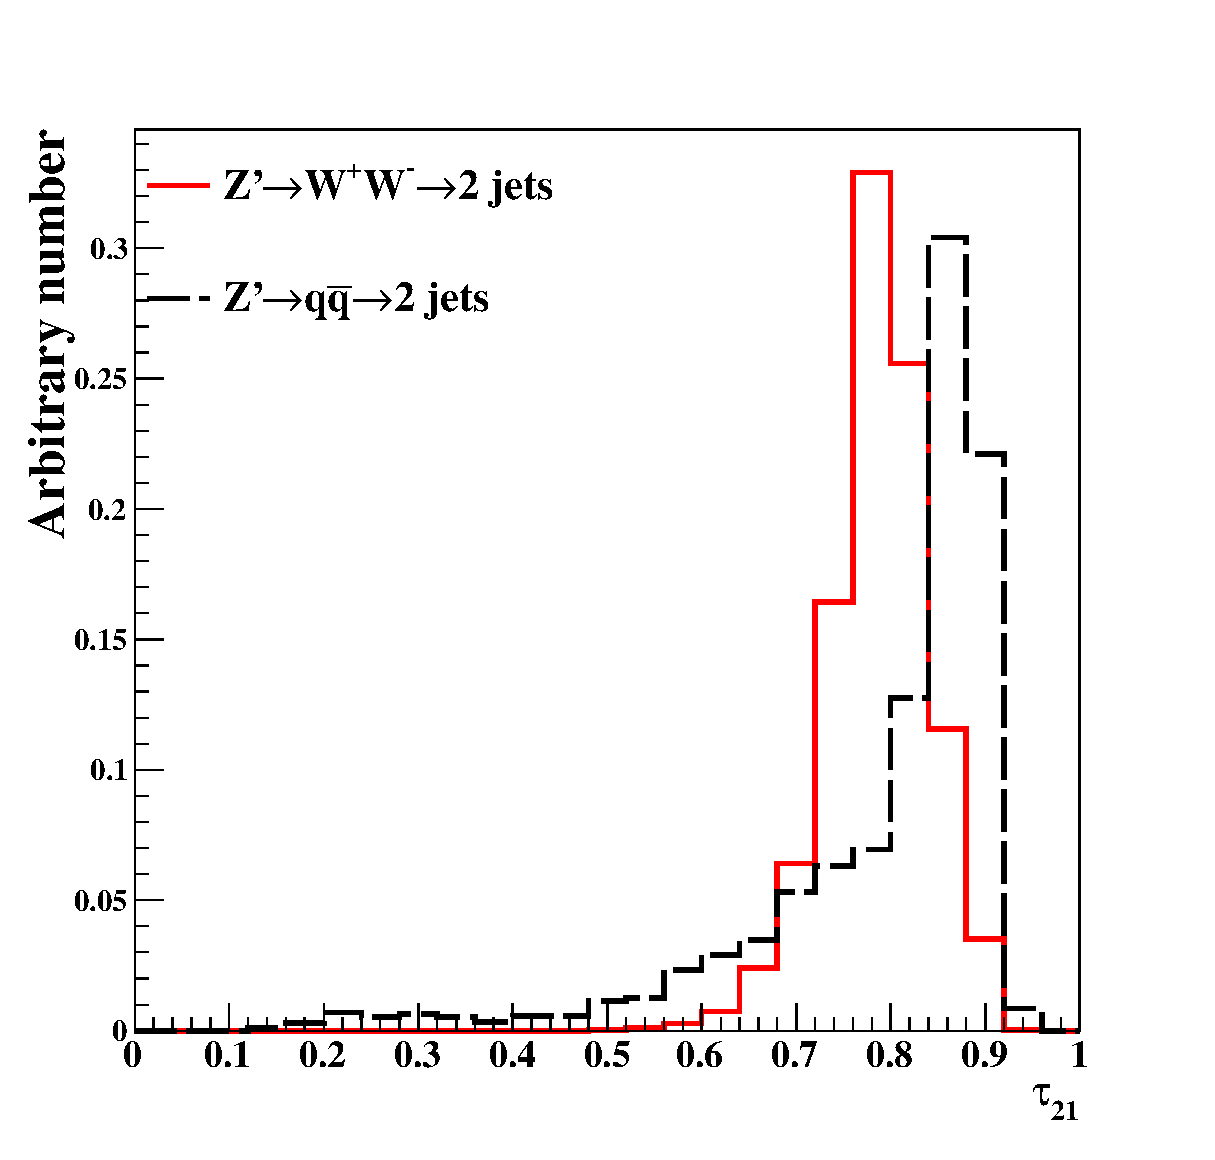
\includegraphics[width=0.3\textwidth]{h_Tau_C/Dis_Rawhit_05GeV_009_tau21_20tev_04_after_cut_Man_25_no_UOF_new_75pa_for_paper.eps}
   }
   \subfigure[1$\times$1 (cm$^2$)] {
   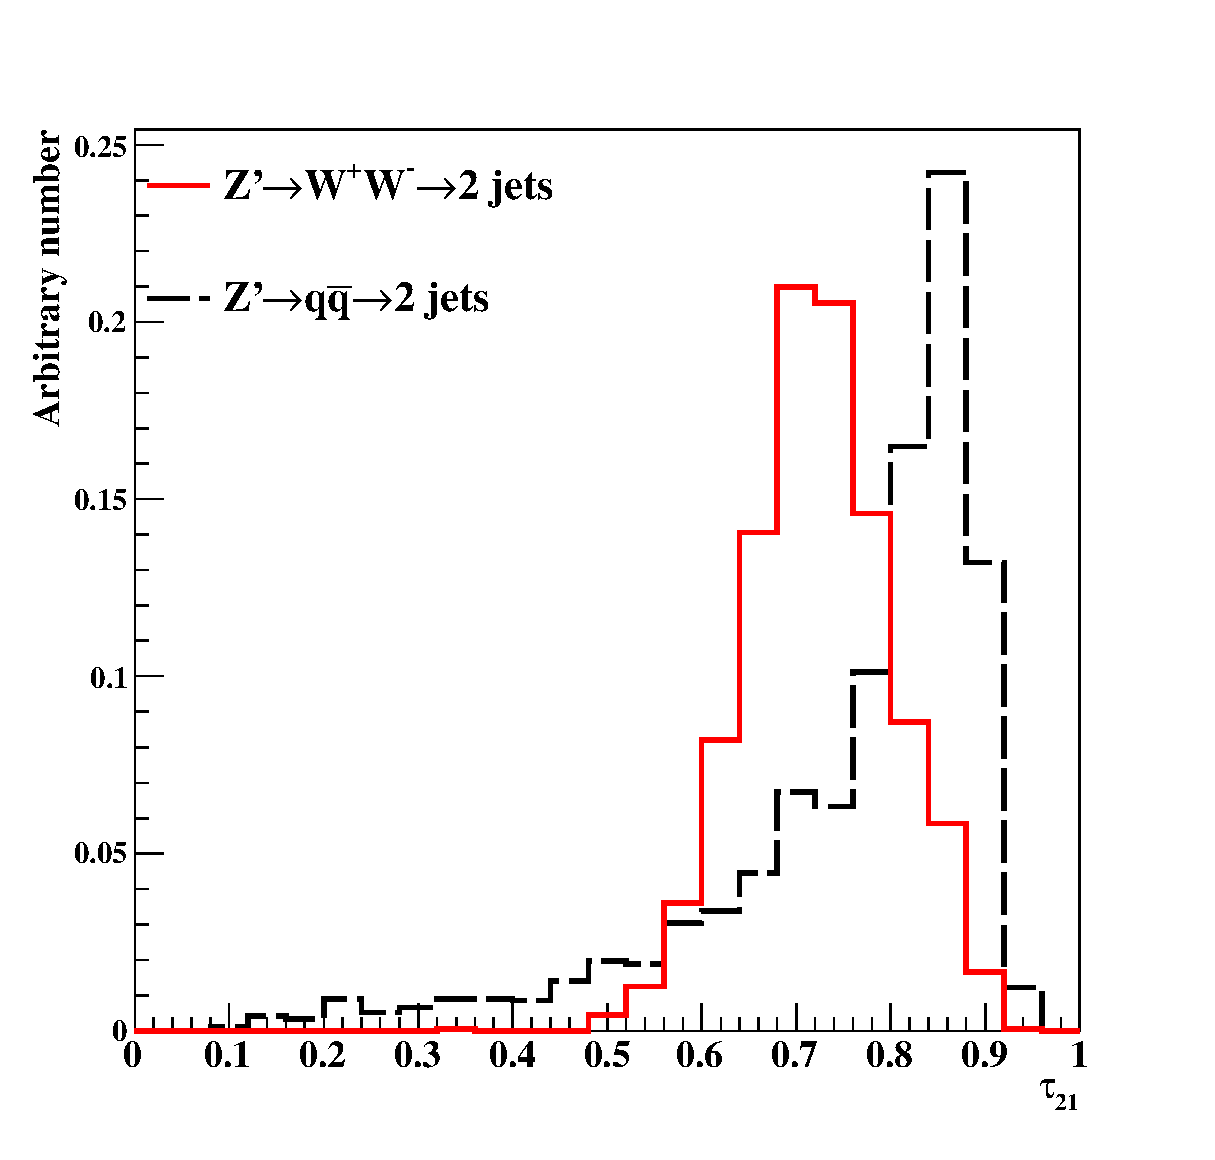
\includegraphics[width=0.3\textwidth]{h_Tau_C/Dis_Rawhit_05GeV_012_tau21_20tev_04_after_cut_Man_25_no_UOF_new_75pa_for_paper.eps}
   }
\end{center}
\caption{Distributions of $\tau_{21}$ in 20~TeV energy collision for different 
detector sizes. Cell sizes in 20$\times$20, 5$\times$5, and 1$\times$1~cm$^2$ 
are shown here. \label{fig:Rawhit_05GeV_tau21_Dis}}
\end{figure}

\begin{figure}
\begin{center}
   \subfigure[$Z'$ (5 TeV)] {
   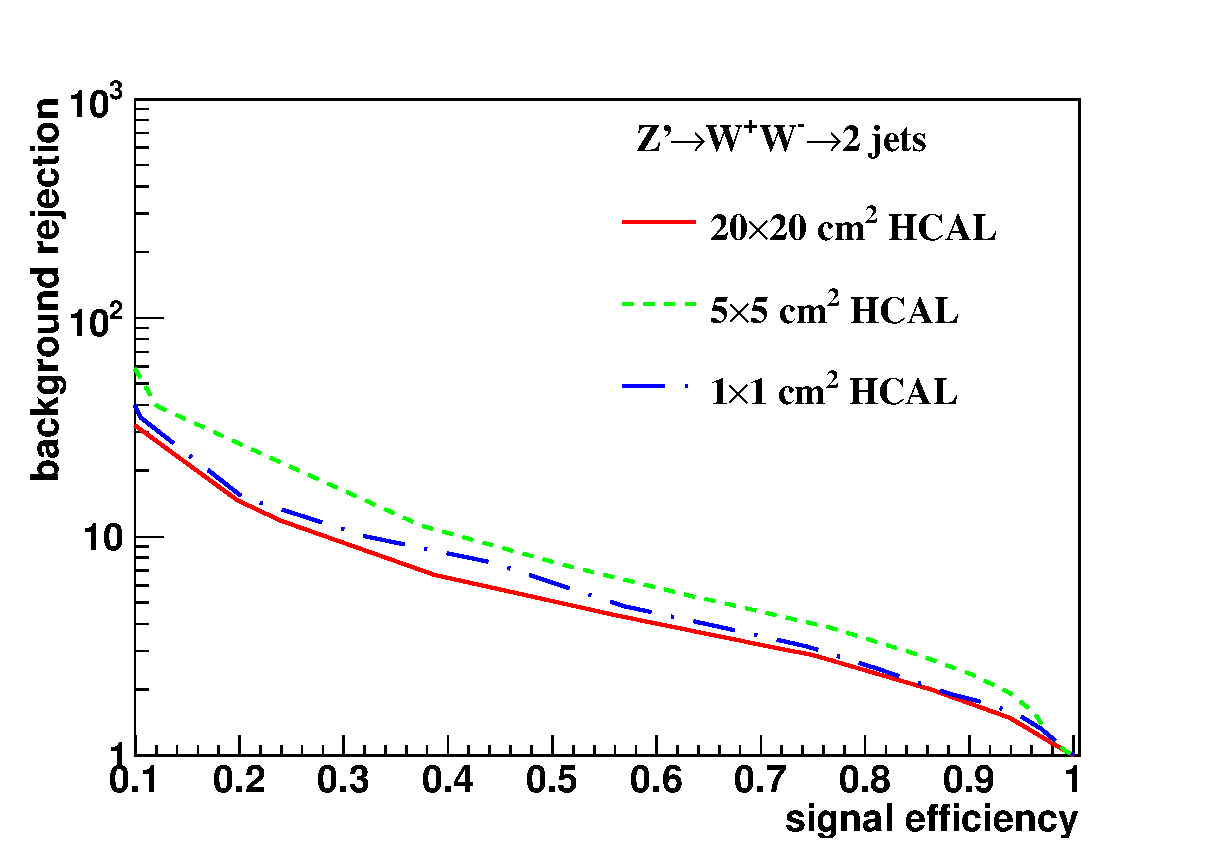
\includegraphics[width=0.43\textwidth]{ROC_Tau_C/Rawhit_05GeV_tau21_5tev_eff_1_New2_after_cut_25bins_no_UOF_new_75pa.eps}
   }
   \subfigure[$Z'$ (10 TeV)] {
   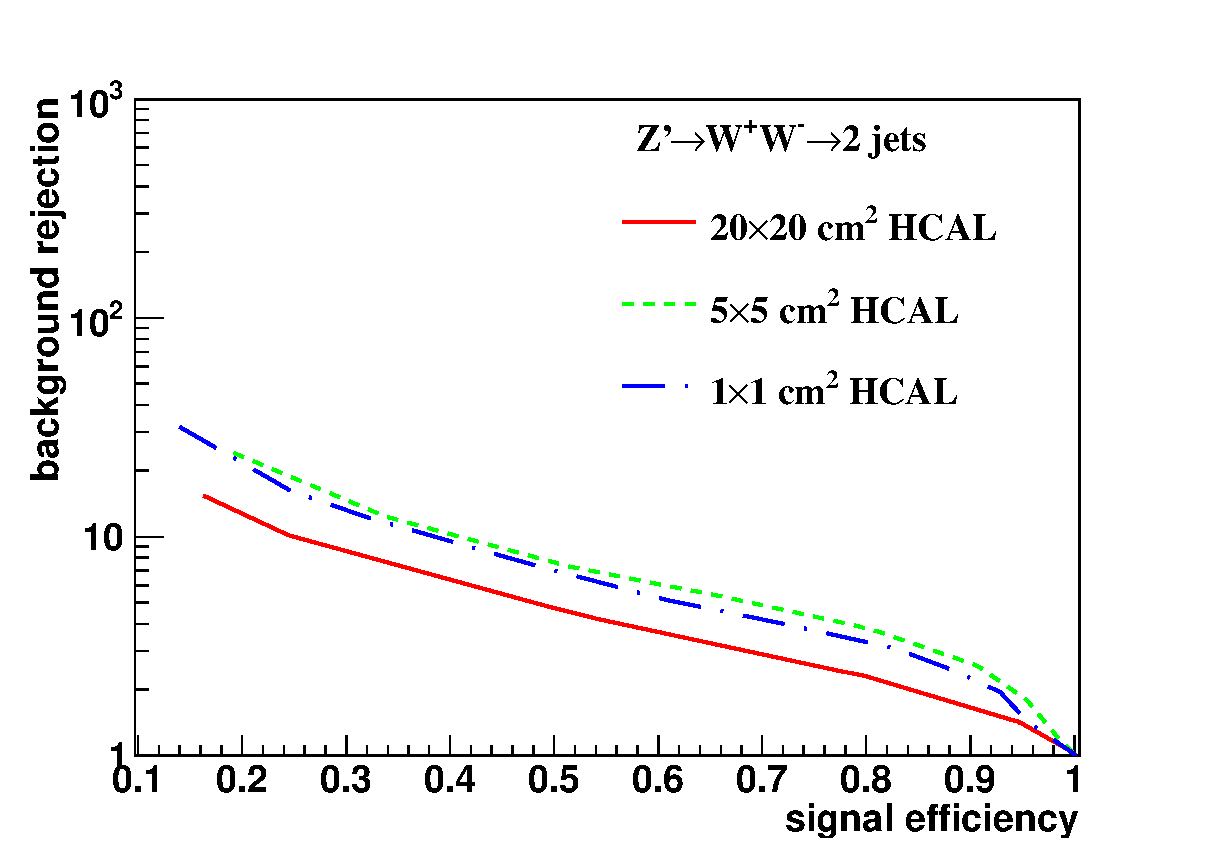
\includegraphics[width=0.43\textwidth]{ROC_Tau_C/Rawhit_05GeV_tau21_10tev_eff_1_New2_after_cut_25bins_no_UOF_new_75pa.eps}
   }
   \subfigure[$Z'$ (20 TeV)] {
   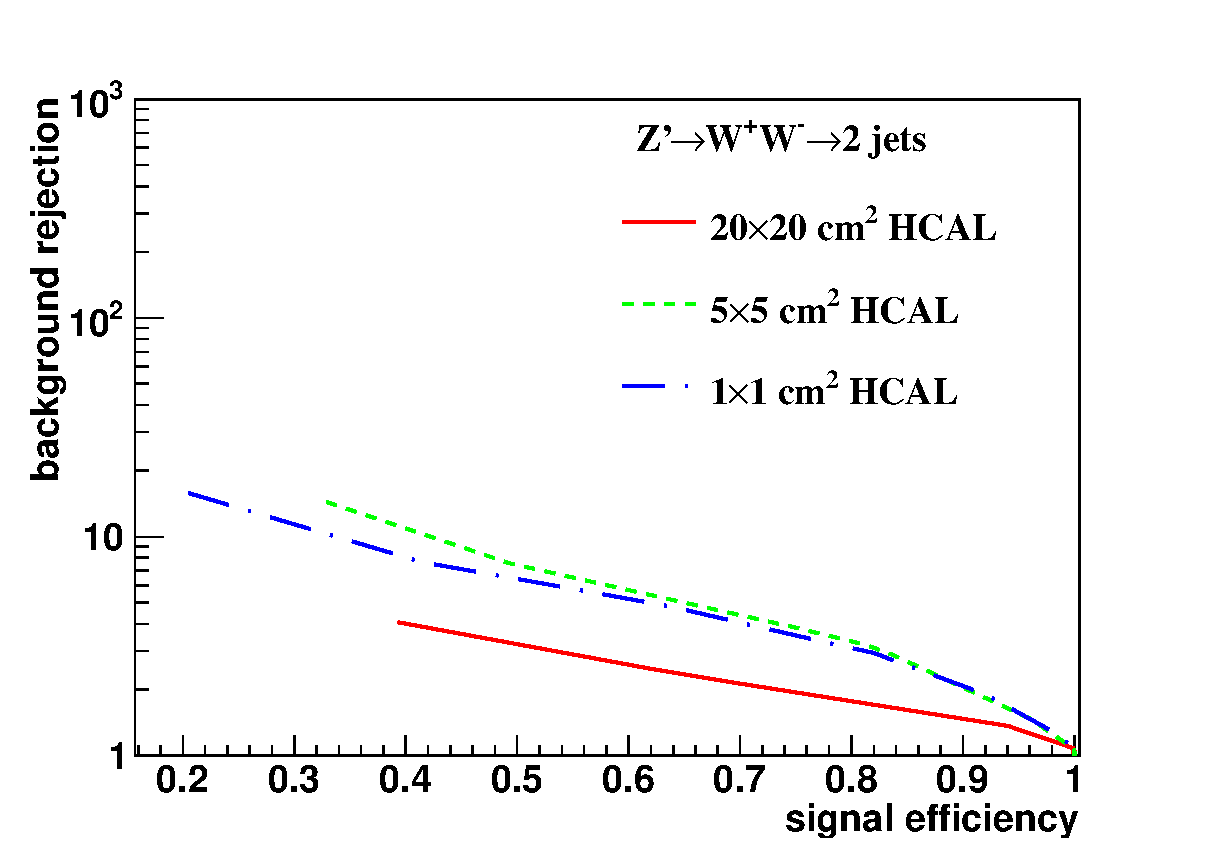
\includegraphics[width=0.43\textwidth]{ROC_Tau_C/Rawhit_05GeV_tau21_20tev_eff_1_New2_after_cut_25bins_no_UOF_new_75pa.eps}
   }
   \subfigure[$Z'$ (40 TeV)] {
   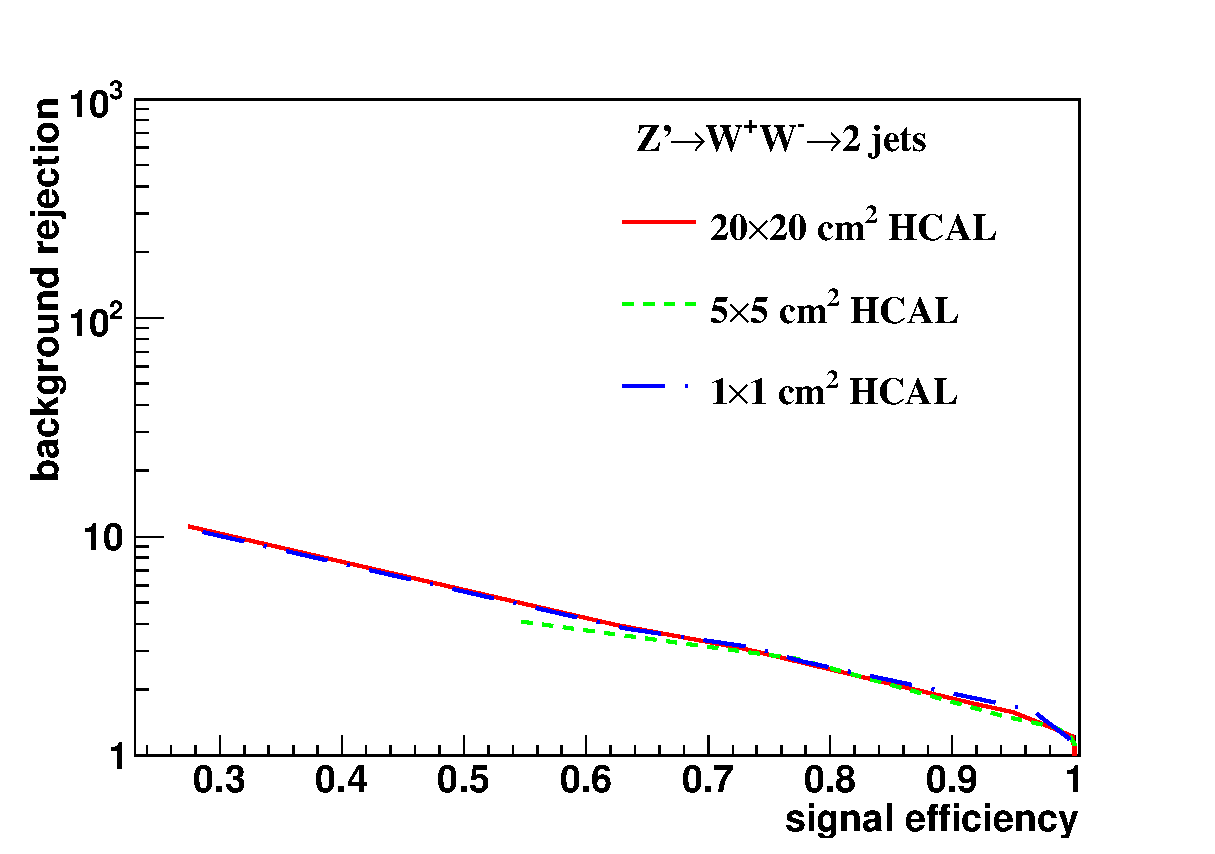
\includegraphics[width=0.43\textwidth]{ROC_Tau_C/Rawhit_05GeV_tau21_40tev_eff_1_New2_after_cut_25bins_no_UOF_new_75pa.eps}
   }
\end{center}
\caption{Signal efficiency versus background rejection rate using $\tau_{21}$.
The energies of collision at (a) 5, (b) 10, (c) 20 and (d) 40~TeV are shown 
here. 
In each figure, the three ROC curves correspond to different detector sizes.
\label{fig:Rawhit_05GeV_tau21_ROC}
}
\end{figure}



%%%%%%%%%% Tau32
%25bins
\begin{figure}
\begin{center}
   \subfigure[20$\times$20 ($cm^2$)] {
   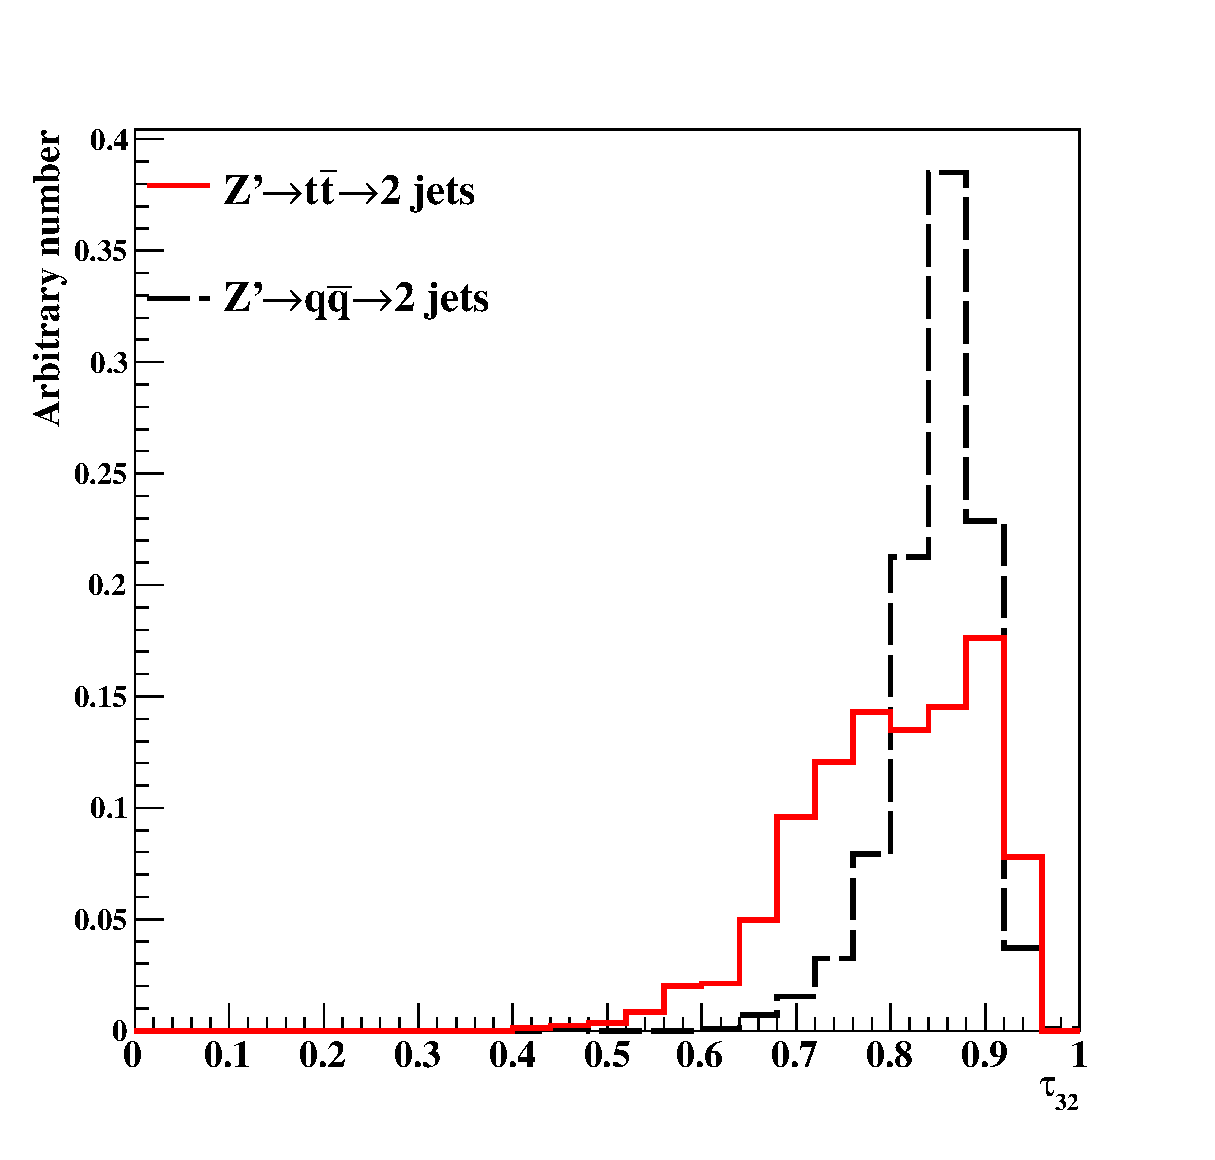
\includegraphics[width=0.3\textwidth]{h_Tau_C/Dis_Rawhit_05GeV_010_tau32_20tev_04_after_cut_Man_25_no_UOF_new_75pa_for_paper.eps}
   }
   \subfigure[5$\times$5 ($cm^2$)] {
   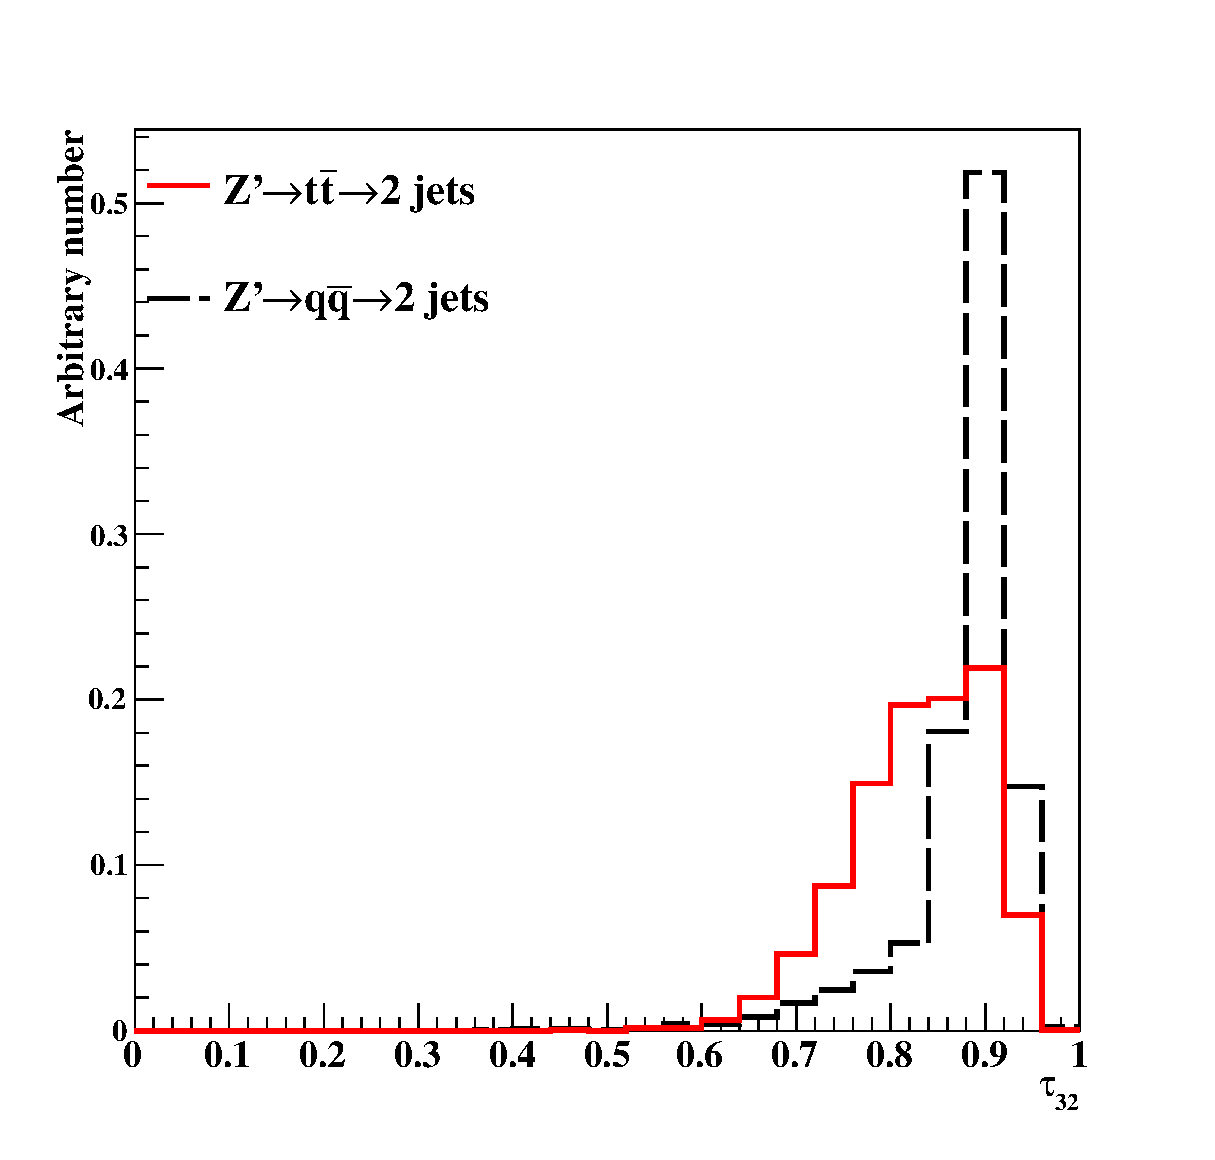
\includegraphics[width=0.3\textwidth]{h_Tau_C/Dis_Rawhit_05GeV_009_tau32_20tev_04_after_cut_Man_25_no_UOF_new_75pa_for_paper.eps}
   }
   \subfigure[1$\times$1 ($cm^2$)] {
   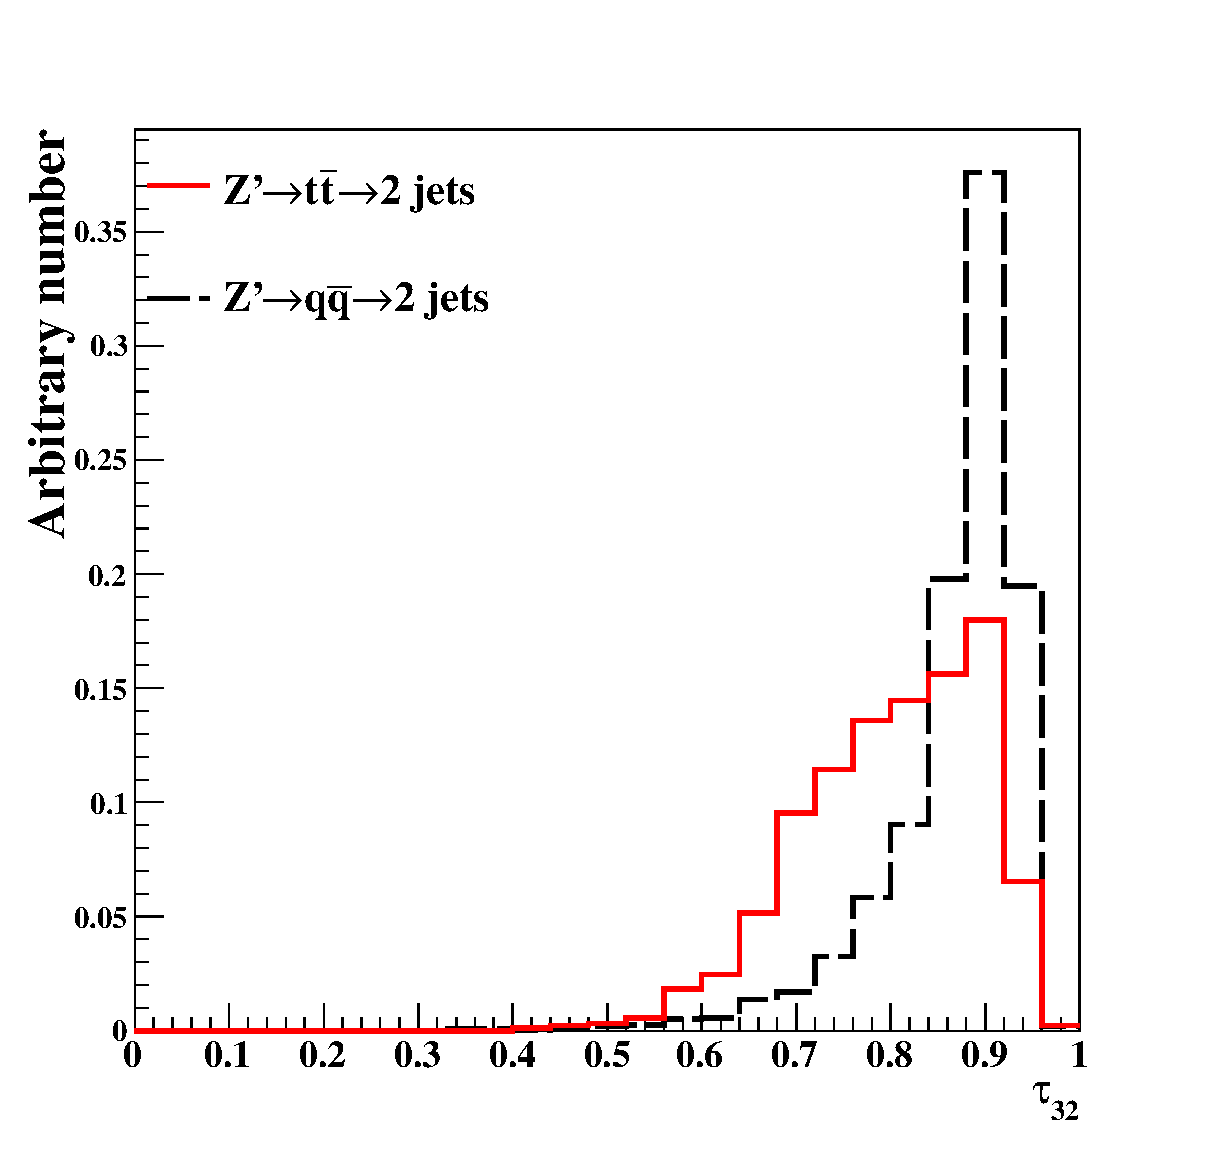
\includegraphics[width=0.3\textwidth]{h_Tau_C/Dis_Rawhit_05GeV_012_tau32_20tev_04_after_cut_Man_25_no_UOF_new_75pa_for_paper.eps}
   }
\end{center}
\caption{Distributions of $\tau_{32}$ in 20 TeV energy collision for different 
detector sizes. Cell sizes in 20$\times$20, 5$\times$5, and 1$\times$1~cm$^2$ 
are shown here.
\label{fig:Rawhit_05GeV_tau32_Dis}
}
\end{figure}

\begin{figure}
\begin{center}
   \subfigure[Z'(5 TeV)] {
   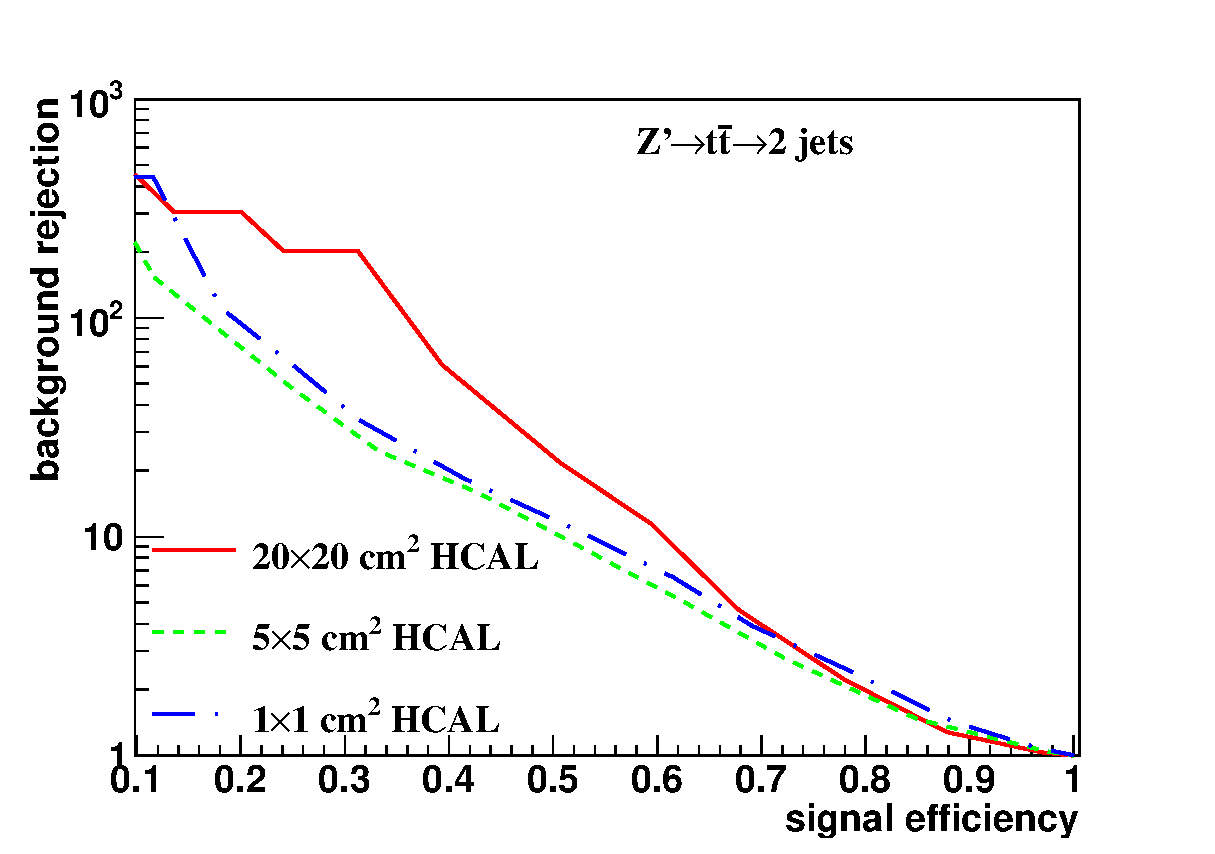
\includegraphics[width=0.43\textwidth]{ROC_Tau_C/Rawhit_05GeV_tau32_5tev_eff_1_New2_after_cut_25bins_no_UOF_new_75pa.eps}\hfill
   }
   \subfigure[Z'(10 TeV)] {
   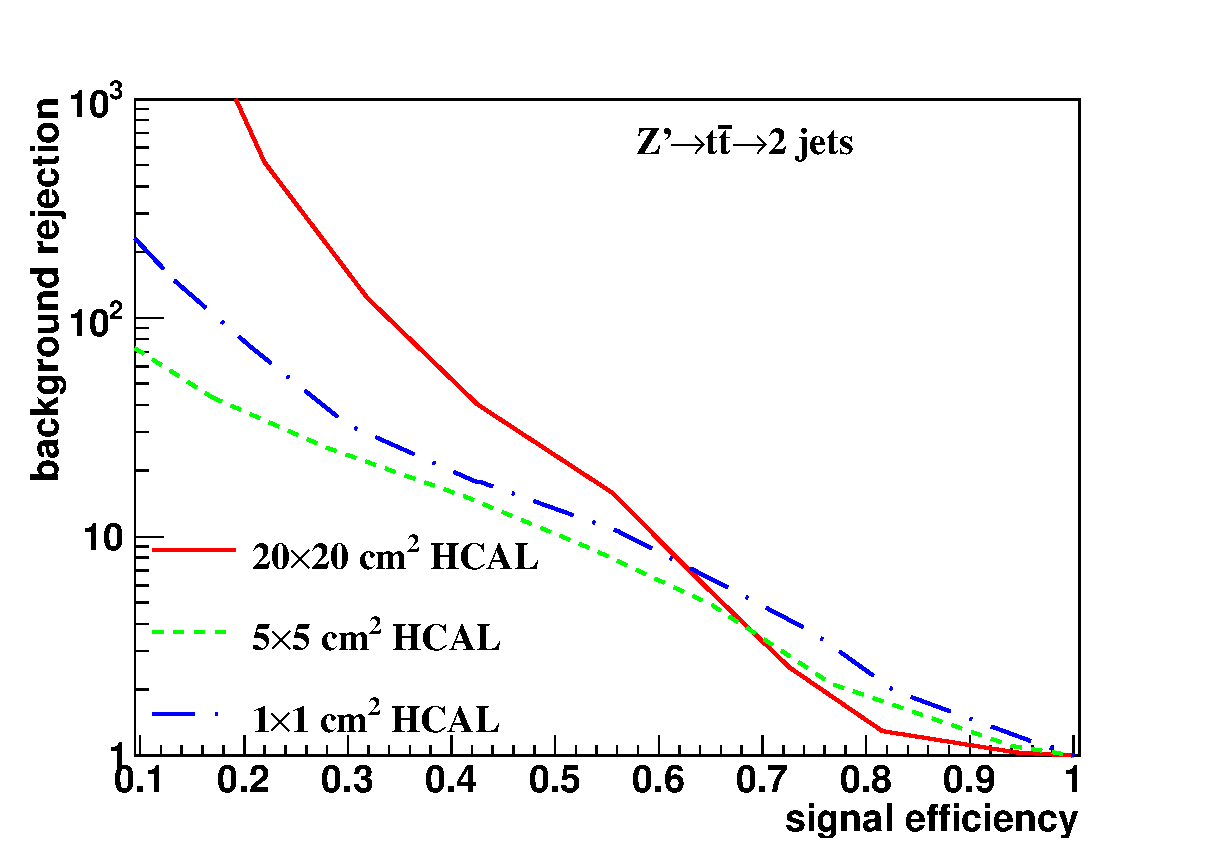
\includegraphics[width=0.43\textwidth]{ROC_Tau_C/Rawhit_05GeV_tau32_10tev_eff_1_New2_after_cut_25bins_no_UOF_new_75pa.eps}
   }
   \subfigure[Z'(20 TeV)] {
   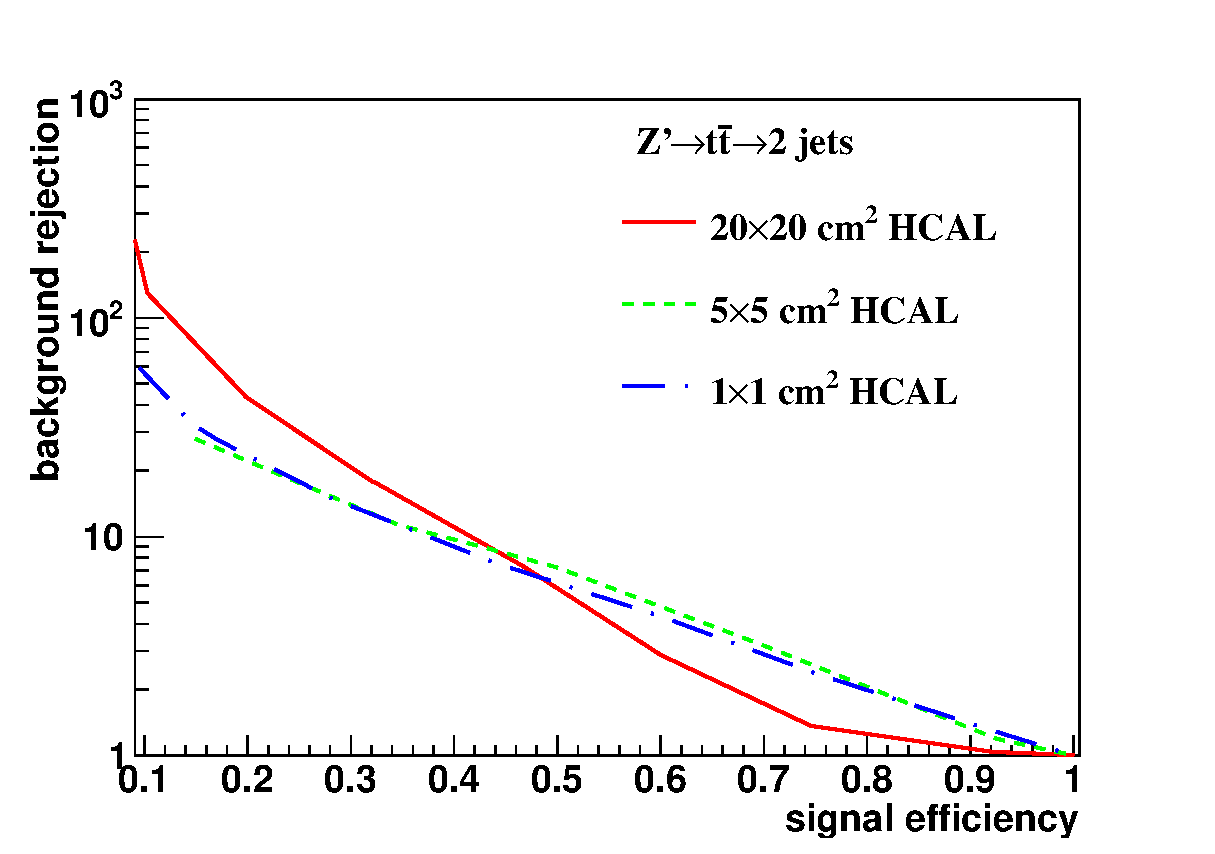
\includegraphics[width=0.43\textwidth]{ROC_Tau_C/Rawhit_05GeV_tau32_20tev_eff_1_New2_after_cut_25bins_no_UOF_new_75pa.eps}
   }
   \subfigure[Z'(40 TeV)] {
   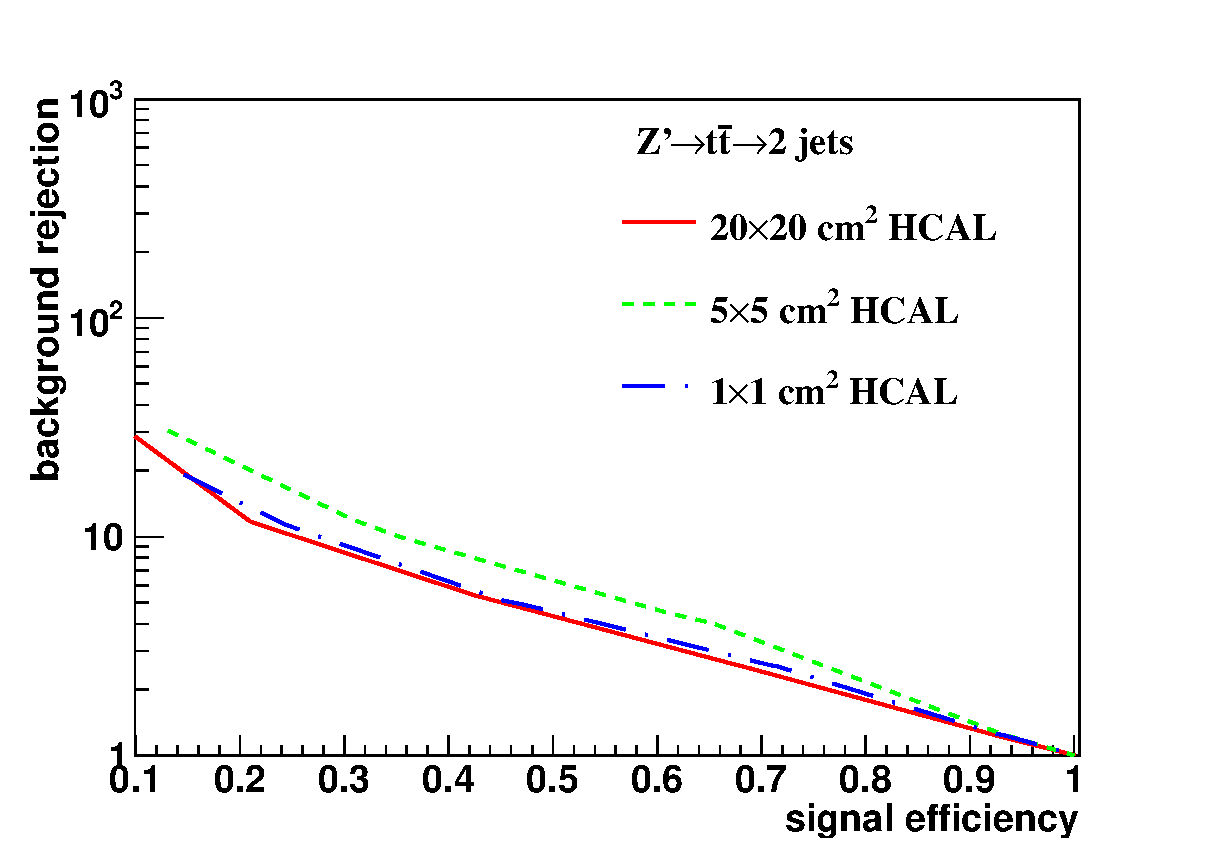
\includegraphics[width=0.43\textwidth]{ROC_Tau_C/Rawhit_05GeV_tau32_40tev_eff_1_New2_after_cut_25bins_no_UOF_new_75pa.eps}
   }
\end{center}
\caption{Signal efficiency versus background rejection rate using $\tau_{32}$. 
The energies of collision at (a) 5, (b) 10, (c) 20 and (d) 40~TeV are shown 
here. In each figure, the three ROC curves correspond to different detector 
sizes.
\label{fig:Rawhit_05GeV_tau32_ROC}
}
\end{figure}


%%%%%%%%%%%%%%% c2b1
%25bins 
\begin{figure}
\centering
\begin{center}
   \subfigure[20$\times$20 ($cm^2$)] {
   \centering
   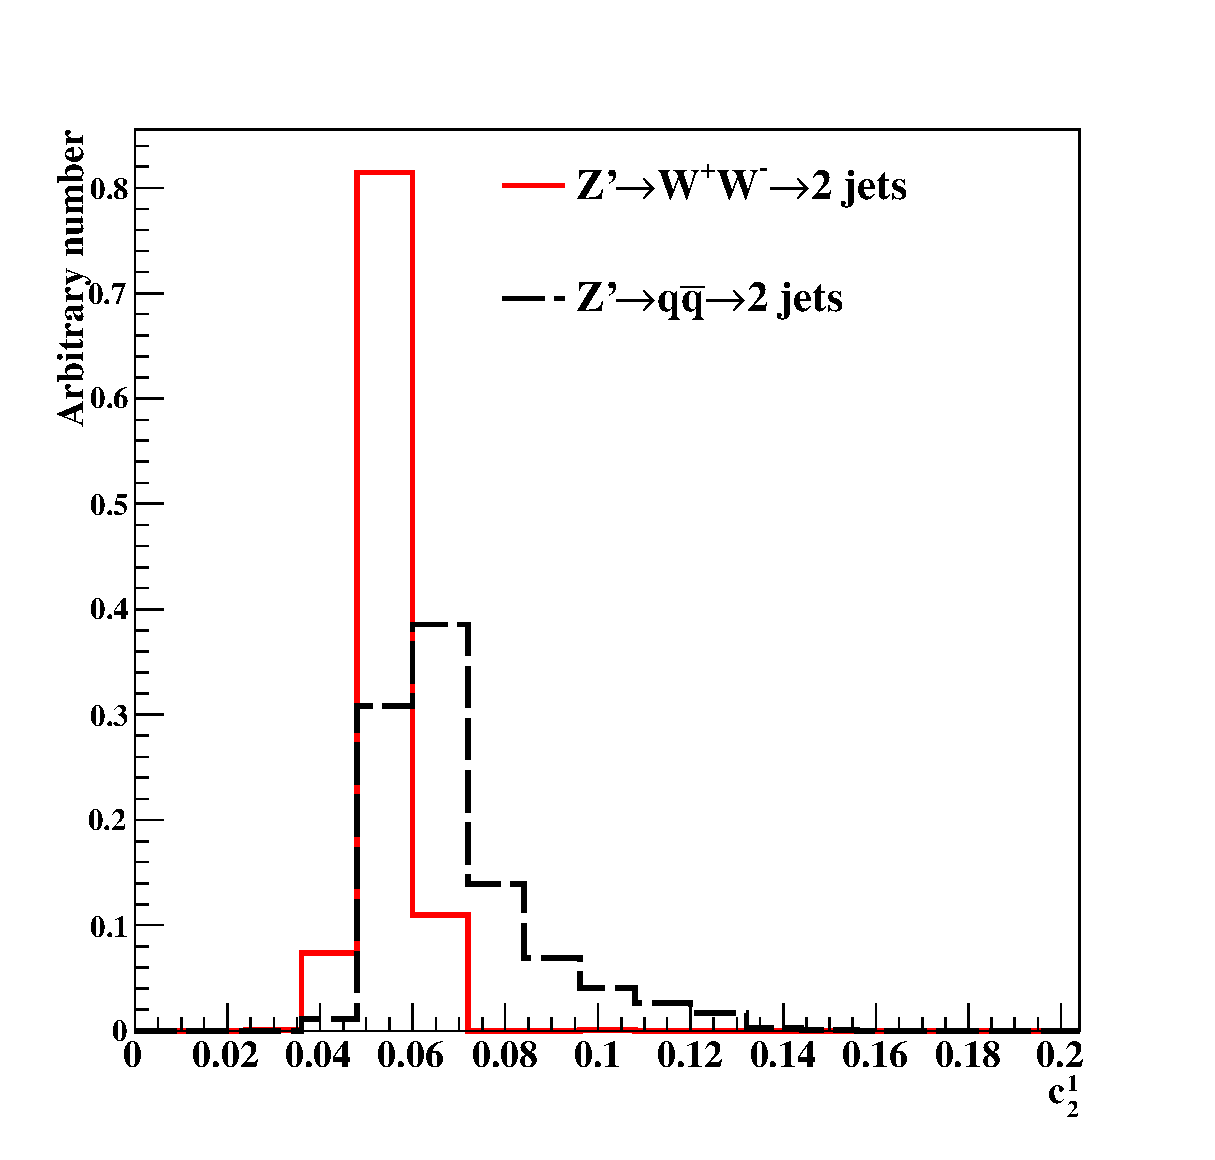
\includegraphics[width=0.3\textwidth]{h_Tau_C/Dis_Rawhit_05GeV_010_c2b1_20tev_04_after_cut_Man_25_no_UOF_new_75pa_for_paper.eps}
   }
   \subfigure[5$\times$5 ($cm^2$)] {
   \centering
   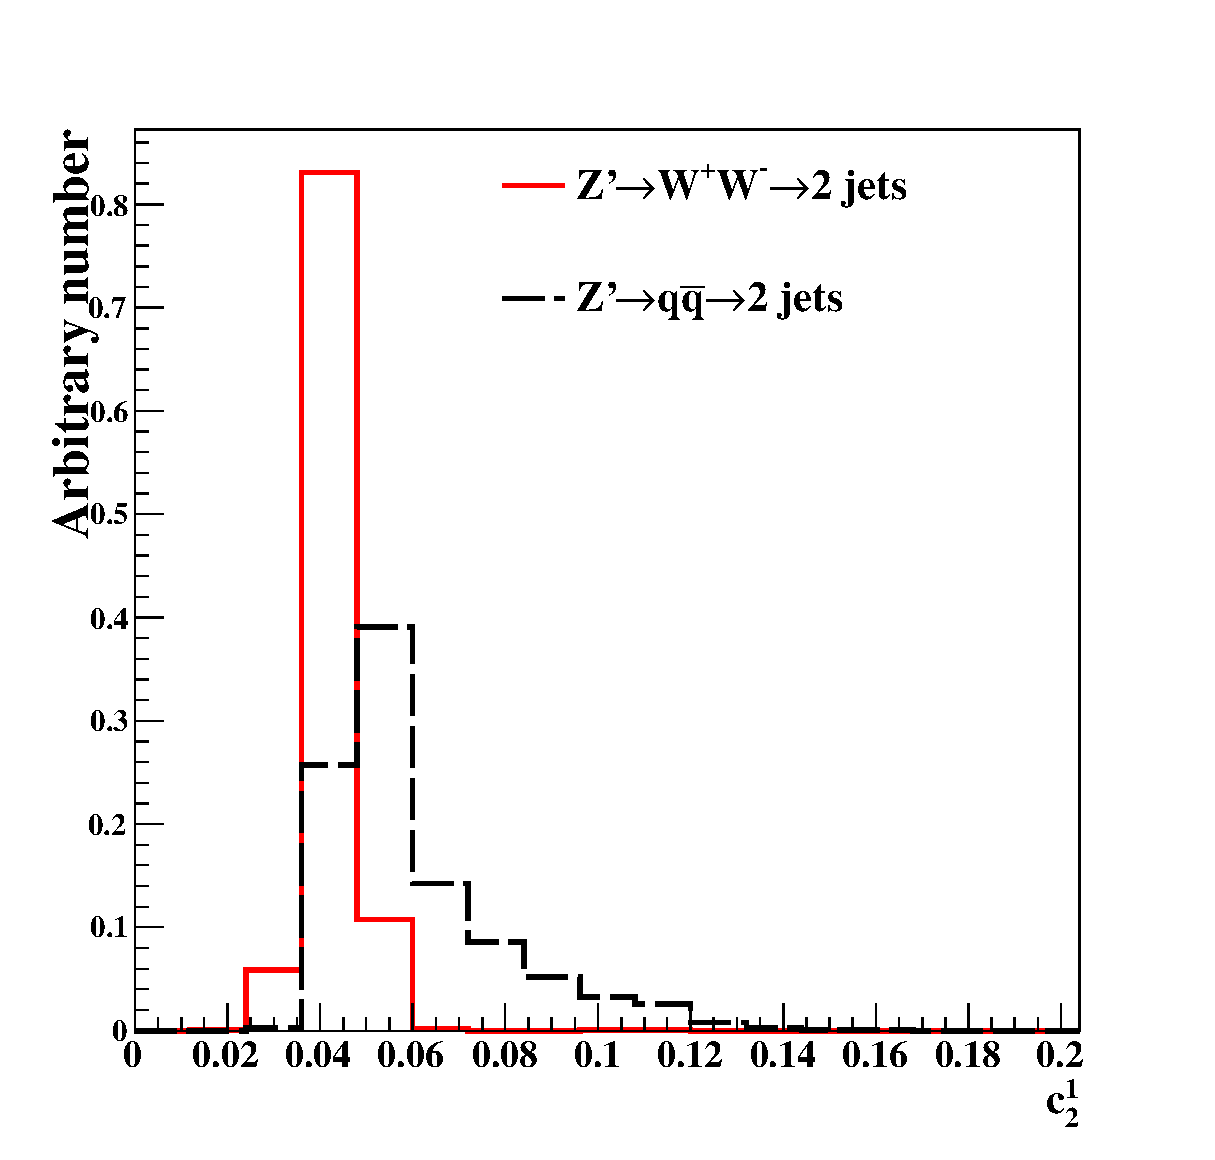
\includegraphics[width=0.3\textwidth]{h_Tau_C/Dis_Rawhit_05GeV_009_c2b1_20tev_04_after_cut_Man_25_no_UOF_new_75pa_for_paper.eps}
   }
   \subfigure[1$\times$1 ($cm^2$)] {
   \centering
   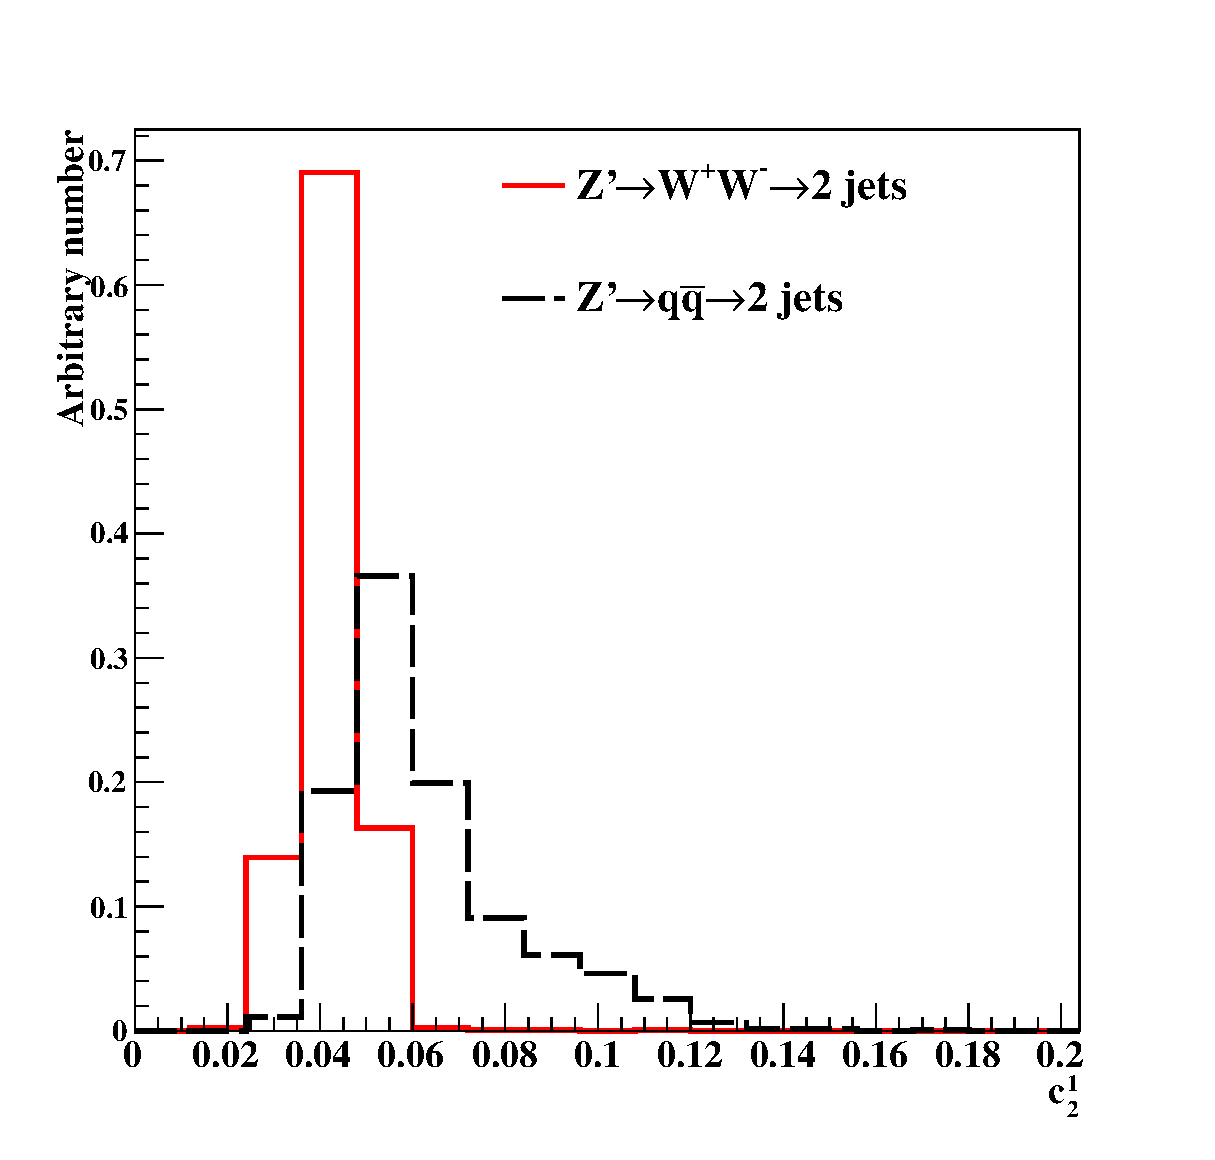
\includegraphics[width=0.3\textwidth]{h_Tau_C/Dis_Rawhit_05GeV_012_c2b1_20tev_04_after_cut_Man_25_no_UOF_new_75pa_for_paper.eps}
   }
\end{center}
\caption{Distributions of $C_2^1$ in 20~TeV energy collision for different 
detector sizes. Cell sizes in 20$\times$20, 5$\times$5, and 1$\times$1~cm$^2$ 
are shown here.}
\label{fig:Rawhit_05GeV_c2b1_Dis}
\end{figure}

\begin{figure}
\begin{center}
   \subfigure[Z'(5 TeV)] {
   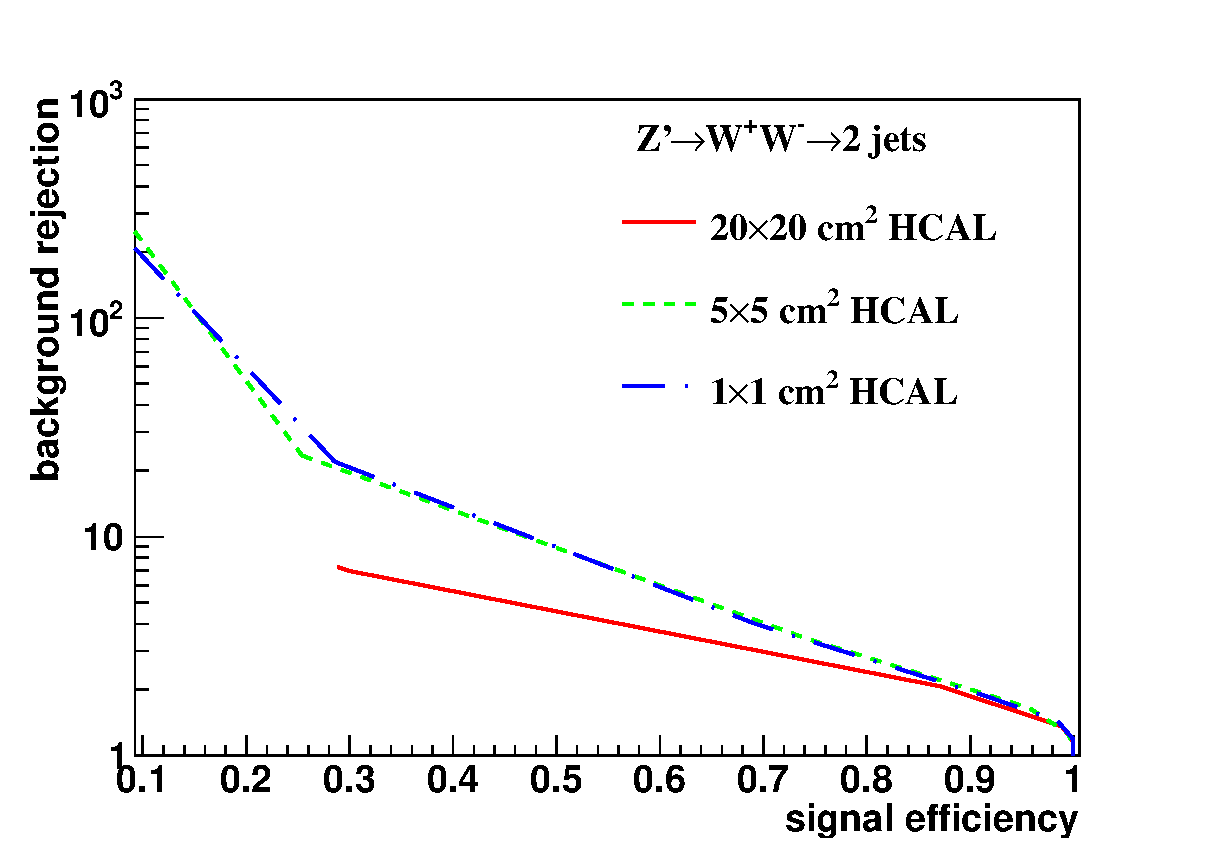
\includegraphics[width=0.43\textwidth]{ROC_Tau_C/Rawhit_05GeV_c2b1_5tev_eff_1_New2_after_cut_25bins_no_UOF_new_75pa.eps}\hfill
   }
   \subfigure[Z'(10 TeV)] {
   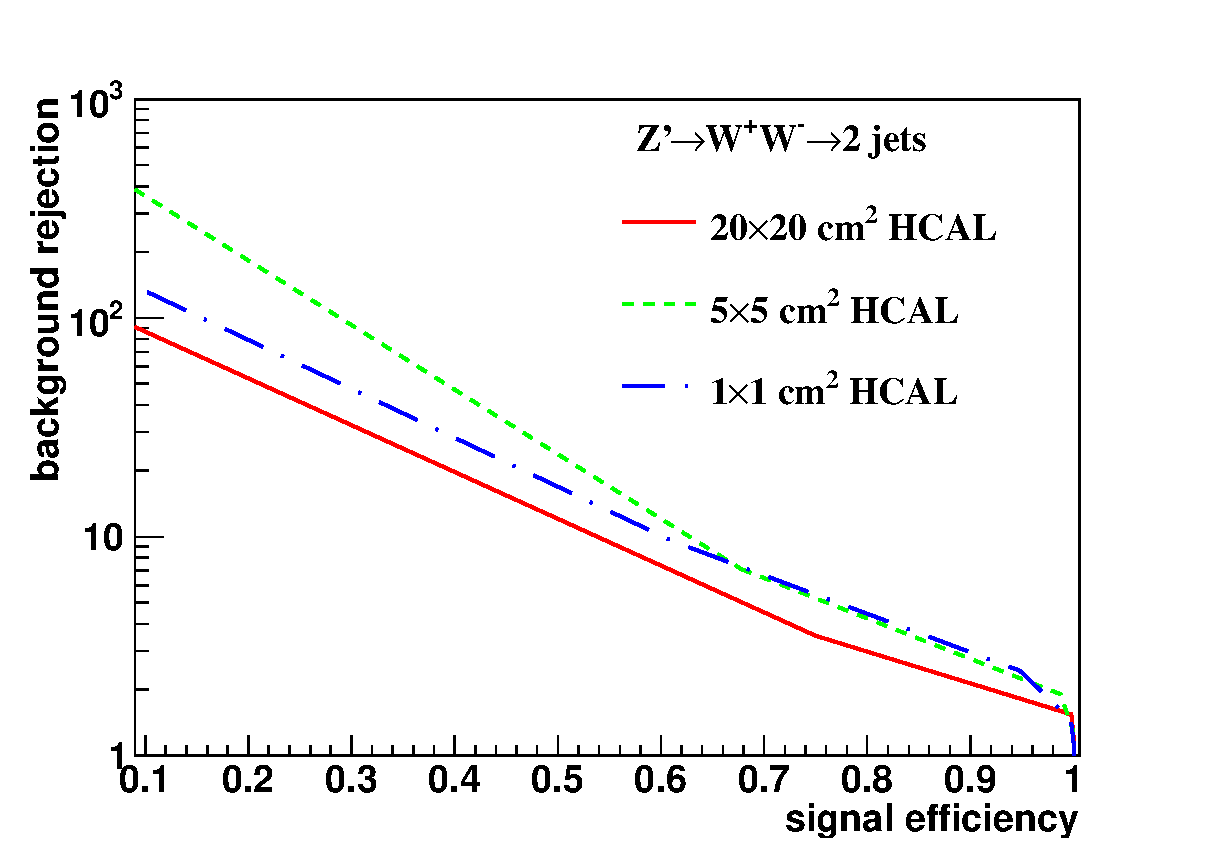
\includegraphics[width=0.43\textwidth]{ROC_Tau_C/Rawhit_05GeV_c2b1_10tev_eff_1_New2_after_cut_25bins_no_UOF_new_75pa.eps}
   }
   \subfigure[Z'(20 TeV)] {
   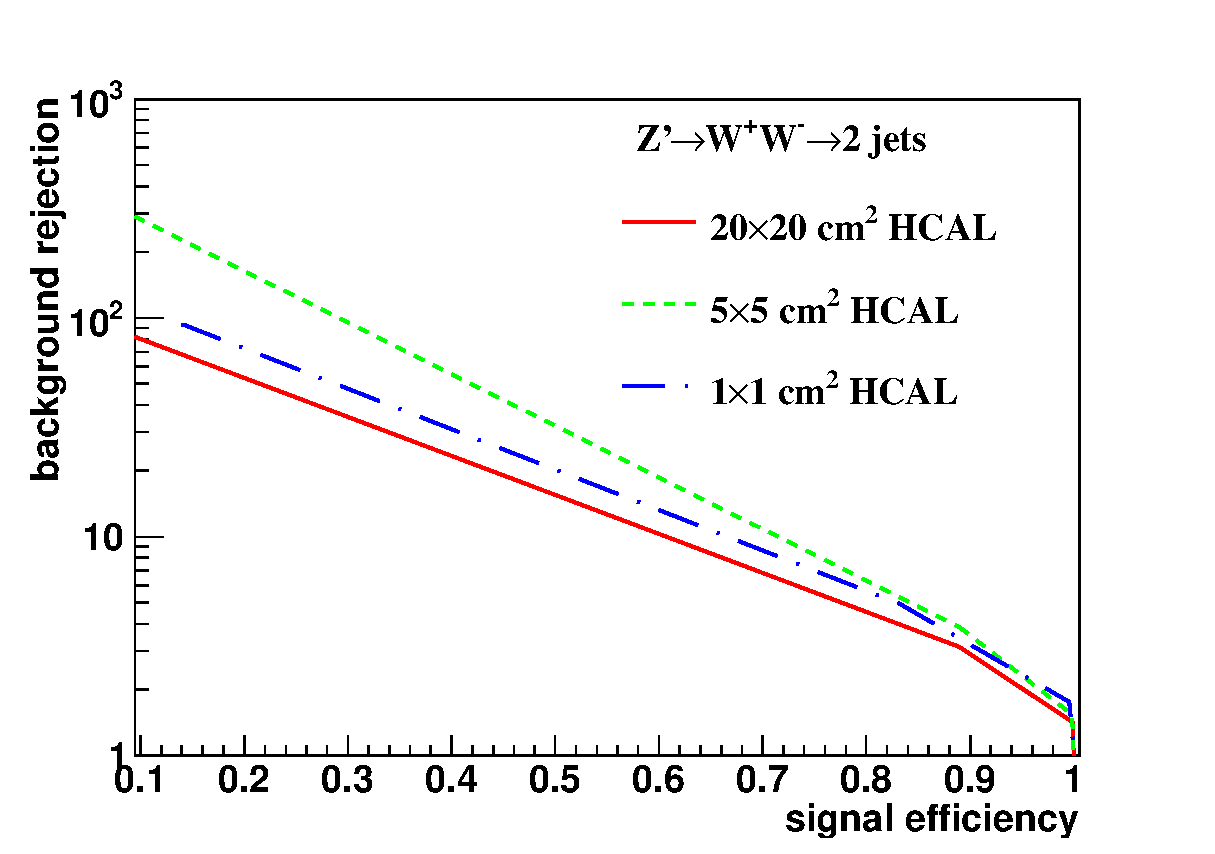
\includegraphics[width=0.43\textwidth]{ROC_Tau_C/Rawhit_05GeV_c2b1_20tev_eff_1_New2_after_cut_25bins_no_UOF_new_75pa.eps}
   }
   \subfigure[Z'(40 TeV)] {
   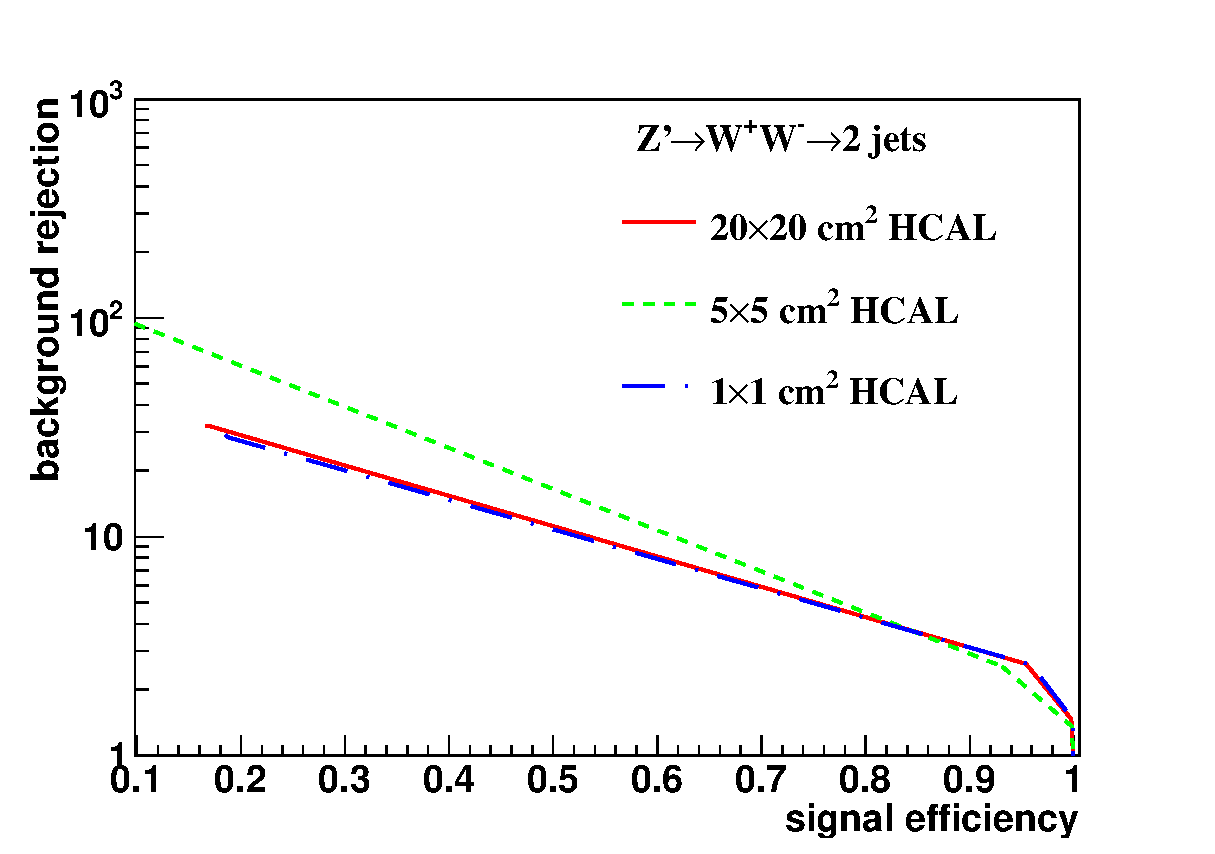
\includegraphics[width=0.43\textwidth]{ROC_Tau_C/Rawhit_05GeV_c2b1_40tev_eff_1_New2_after_cut_25bins_no_UOF_new_75pa.eps}
   }
\end{center}
\caption{Signal efficiency versus background rejection rate using $C_{2}^{1}$. 
The energies of collision at (a) 5, (b) 10, (c) 20, and (d) 40~TeV are shown 
here. In each figure, the three ROC curves correspond to different detector 
sizes.}
\label{fig:Rawhit_05GeV_c2b1_ROC}
\end{figure}



%25bins Mann-Whitney
\begin{figure}
\begin{center}
   \subfigure[$\tau_{21}$] {
   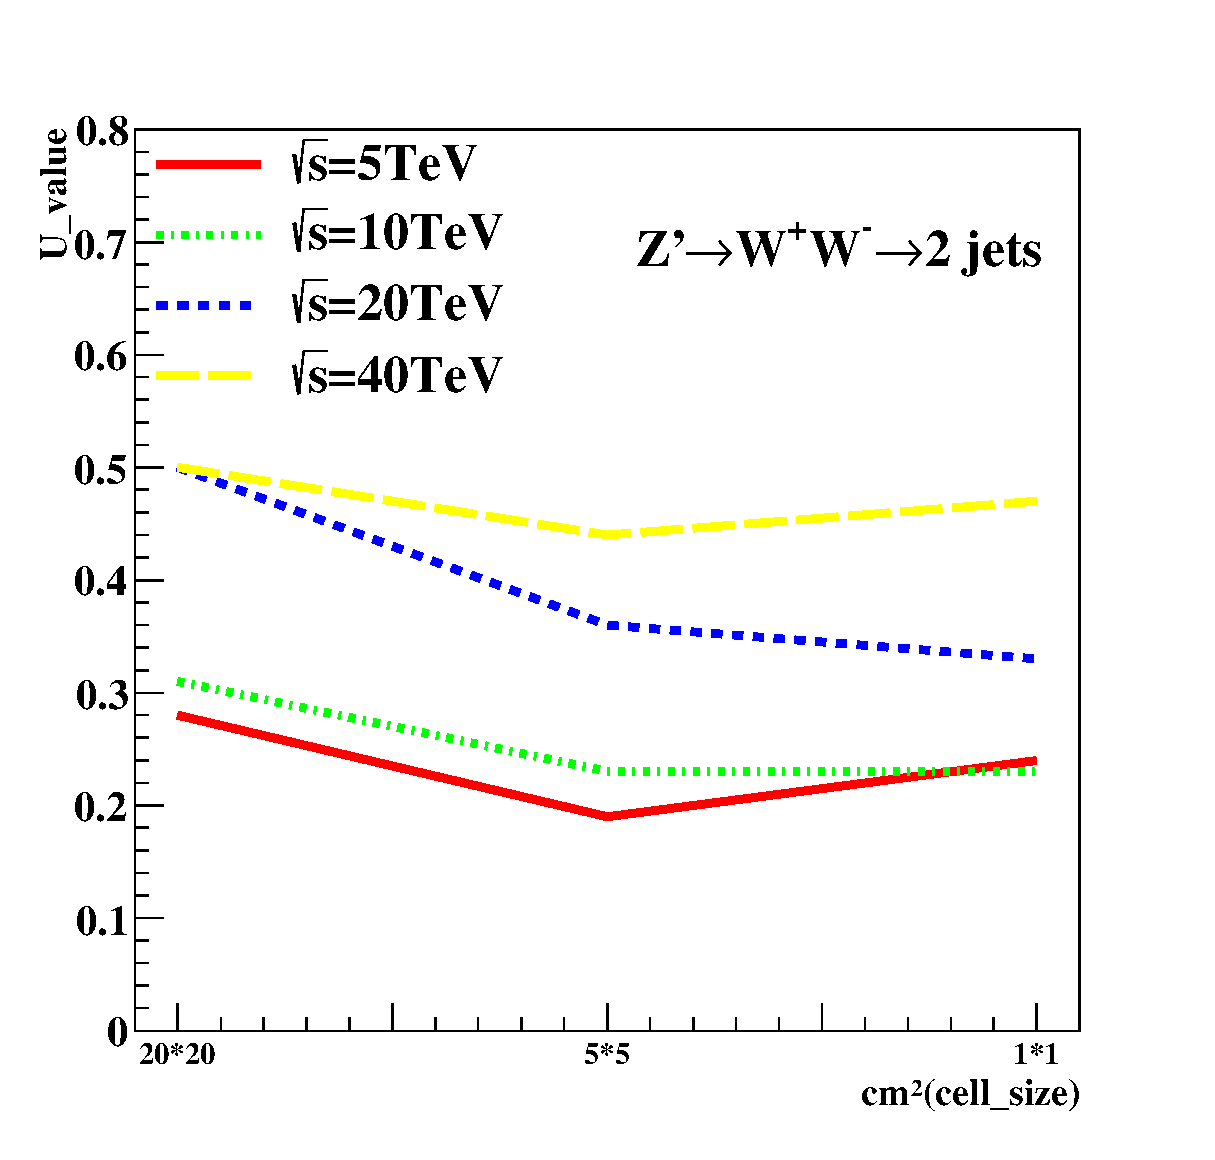
\includegraphics[width=0.3\textwidth]{Mann_Sum/raw_05_tau21_summary_U_after_cut_25bins_no_UOF_new_75pa.eps}\hfill
   }
   \subfigure[$\tau_{32}$ ] {
   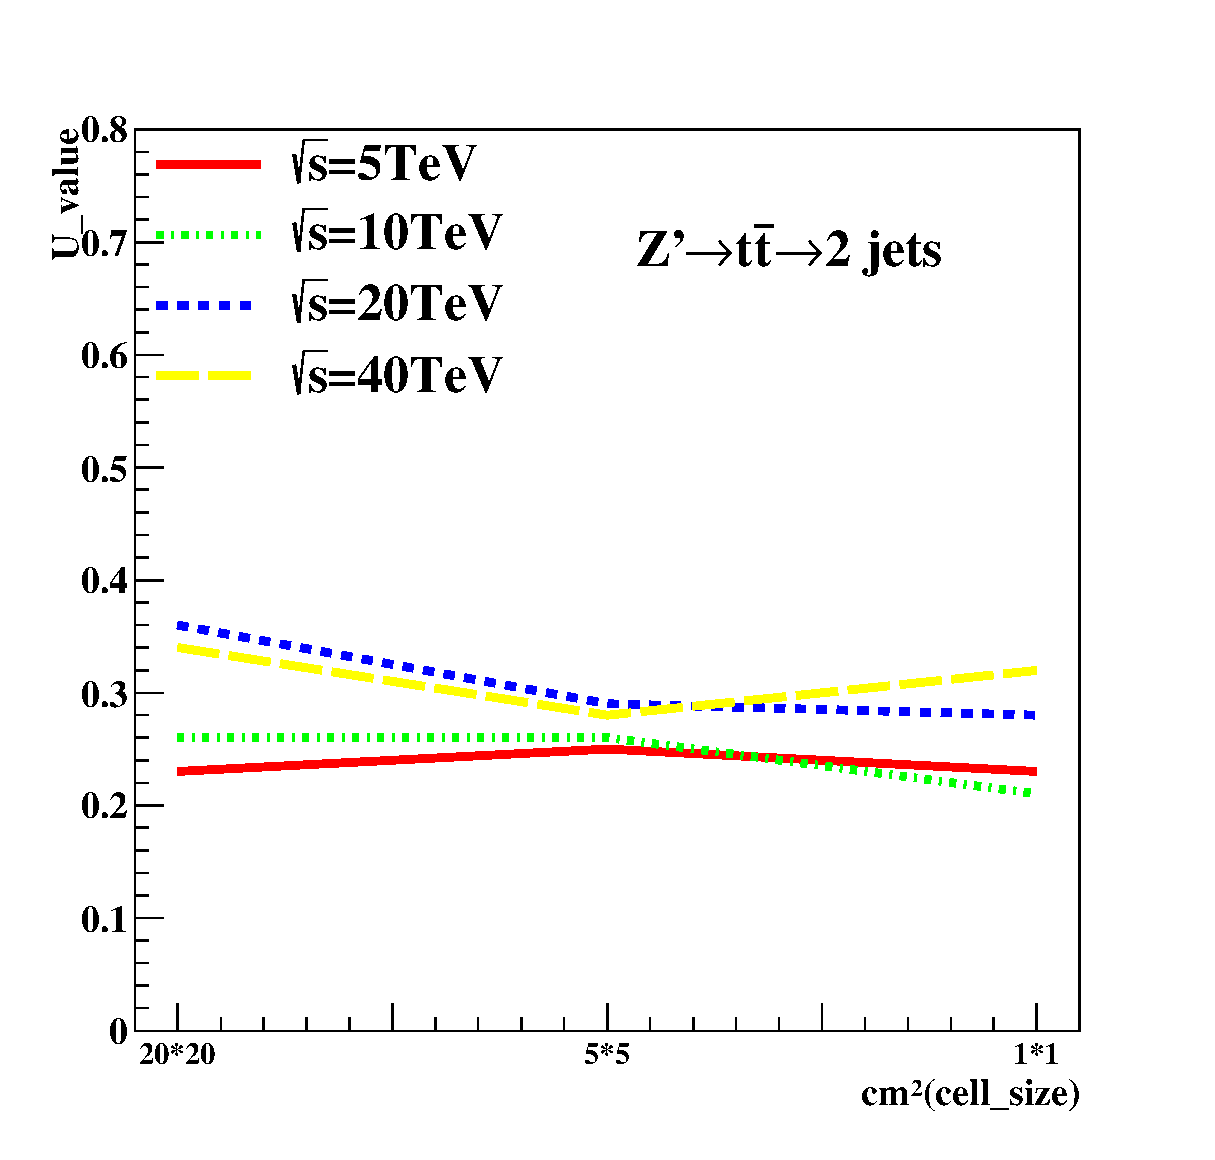
\includegraphics[width=0.3\textwidth]{Mann_Sum/raw_05_tau32_summary_U_after_cut_25bins_no_UOF_new_75pa.eps}
   }
   \subfigure[$C_2^{(1)}$] {
   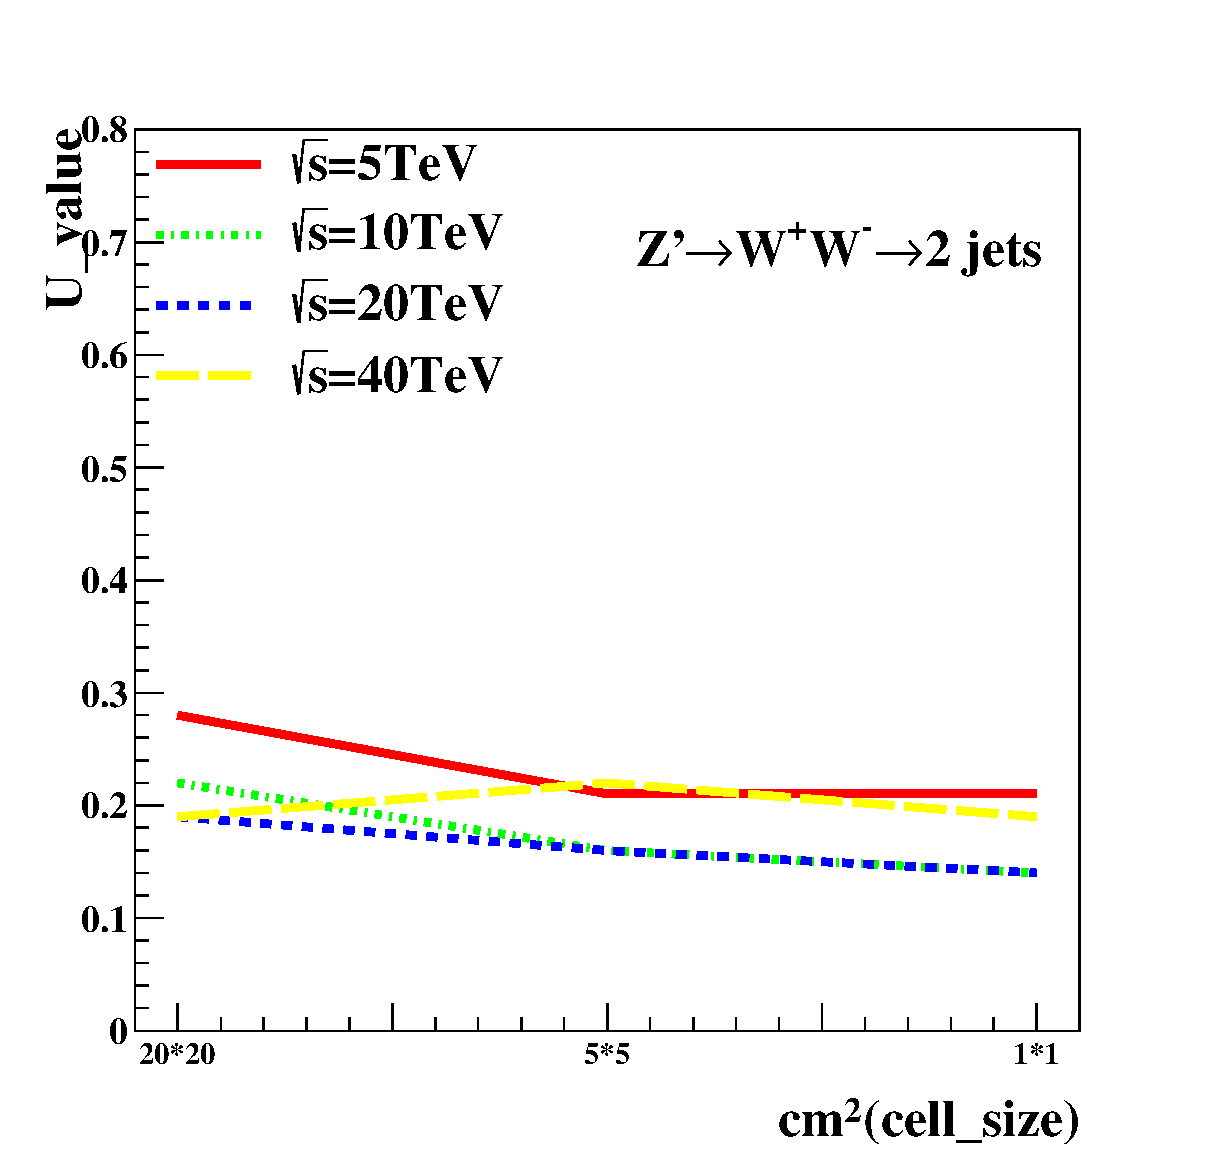
\includegraphics[width=0.3\textwidth]{Mann_Sum/raw_05_c2b1_summary_U_after_cut_25bins_no_UOF_new_75pa.eps}
   }
   \end{center}
\caption{The Mann-Whitney U values for $\tau_{21}$, $\tau_{32}$, and $C_2^{(1)}$ 
reconstructed with different collision energies and detector cell sizes. }
\label{fig:Rawhit_05GeV_total_Mann}
\end{figure}




